\documentclass[master=wit,british,fleqn]{misc/kulemt}

%%%%%%%%%%%%%%%%
%%% PACKAGES %%%
%%%%%%%%%%%%%%%%

%\usepackage{ucs}
\usepackage[TS1,T1]{fontenc}
\usepackage{amsmath}
\usepackage{amsthm}
\usepackage{dsfont}
\usepackage{amsfonts}
\usepackage{amssymb}
\usepackage{mathtools}
\usepackage{tikz}
\usepackage[framemethod=tikz]{mdframed}
\usepackage{microtype}
\usepackage{textcomp}
\usepackage[pdfusetitle,plainpages=false]{hyperref}

%packages spéciaux
%\usepackage{fullpage}
\usepackage{mathrsfs}
%\usepackage{numprint}
\usepackage{graphicx}
\usepackage{float}
\usepackage{wrapfig}
\usepackage[font=small,labelfont=sc]{caption}
\usepackage{makecell}
\usepackage{array}
\usepackage{csquotes}
\usepackage[boxed]{algorithm2e}

\usepackage[numbered,framed,autolinebreaks]{misc/mcode}

%% FONTS
\usepackage[lf]{Baskervaldx} % lining figures
\usepackage[bigdelims,vvarbb]{newtxmath} % math italic letters from Nimbus Roman
\usepackage[cal=boondoxo]{mathalfa} % mathcal from STIX, unslanted a bit
\renewcommand*\oldstylenums[1]{\textosf{#1}}
%\usepackage{sfmath}
%\usepackage{sansmathaccent}
%\usepackage{beramono}

\usepackage{caption}
\usepackage{subcaption}

%% STYLE
\pagestyle{headings}
\usepackage{misc/slashbox}
\usepackage{placeins} % permet d'utiliser \FloatBarrier et donc d'imposer le placement des images dans une section donnée.
\usepackage{multirow}

\newcommand\scalemath[2]{\scalebox{#1}{\mbox{\ensuremath{\displaystyle #2}}}}
\newcommand{\HRule}{\rule{\linewidth}{0.5mm}}

\newcommand{\overbar}[1]{\mkern 1.5mu\overline{\mkern-1.5mu#1\mkern-1.5mu}\mkern 1.5mu}

\definecolor{grisclair}{HTML}{F2F2F2}
\lstset{language=Matlab, breaklines=true, backgroundcolor=\color{grisclair} , numbers=left, frame=none, aboveskip=0cm} %, basicstyle=\tiny}

\usepackage{fancyhdr}
%\addto\captionsenglish{\renewcommand{\chaptername}{Assignment}}

%% TABLES
\usepackage{tabularx}
\newcommand\hlineI{\noalign{\hrule height 1.2pt}} % I line 1.2pt
\newcolumntype{I}{!{\vline width 1.2pt}} % I column 1.2pt

%\newcolumntype{L}[1]{>{\raggedright\let\newline\\\arraybackslash\hspace{0pt}}m{#1}}
%\newcolumntype{C}[1]{>{\centering\let\newline\\\arraybackslash\hspace{0pt}}m{#1}}
%\newcolumntype{R}[1]{>{\raggedleft\let\newline\\\arraybackslash\hspace{0pt}}m{#1}}

\newcolumntype{C}[1]{%
 >{\vbox to 2ex\bgroup\vfill\centering\arraybackslash}%
 p{#1}%
 <{\vskip-\baselineskip\vfill\egroup}}

%% SCALED VERBATIM
\usepackage{verbatim}
\usepackage{adjustbox}
\usepackage{fancyvrb}
\newenvironment{myverb}{%
 \VerbatimEnvironment
 \begin{adjustbox}{max width=1\linewidth}
 \begin{BVerbatim}
  }{
  \end{BVerbatim}
 \end{adjustbox}
}

%% PERSONAL COMMANDS
\newcommand{\noteH}[1]{{\color{red} \textit{#1}}}
\newcommand{\norm}[1]{\left\lVert#1\right\rVert}

\newcommand{\secret}[1]{\langle #1 \rangle}
\newcommand{\secretI}[1]{\langle \bar{#1} \rangle}
\newcommand{\secretF}[1]{\langle \tilde{#1} \rangle}


%% OTHERS
\DeclareMathOperator{\tr}{tr}

%% BIBLIOGRAPHY
\usepackage[backend=biber,style=ieee,url=false,dashed=false,doi=false,bibwarn=false,sorting=nyt]{biblatex}
\addbibresource{misc/references.bib}
%\usepackage{cite}

%%%%%%%%%%%%%
%%% SETUP %%%
%%%%%%%%%%%%%

\setup{title={Privacy-friendly machine learning algorithms for intrusion detection systems},
  author={Henri De Plaen},
  promotor={Prof.\,Dr.\,ir.\,Bart~Preneel},
  assessor={Prof.\,Dr.\,ir.\,Sabine~Van~Huffel \and Prof.\,Dr.\,ir.\,Karl~Meerbergen},
  assistant={ Dr.\,Aysajan~Abidin \and Dr.\,Abdelrahaman~Aly}}

\setup{filingcard,
  translatedtitle=,
  udc=621.3,
  shortabstract={In today's information age, the risks and security threats to data are commonplace. Vital enterprise and user information should be protected from uninvited intruders lurking in our systems. Imagine the case where intruders are accessing to sensitive medical, industrial or governmental records using stolen or hacked but valid credentials. Machine learning techniques and algorithms have been used as a tool for intrusion detection in such scenarios. They typically monitor the behavior of the users, detecting anomalies that indicate possible infiltrations.}}

%\setup{font=lm}

%%%%%%%%%%%%%%%%
%%% DOCUMENT %%%
%%%%%%%%%%%%%%%%

\begin{document}

% \begin{preface}
 I would like to thank everybody who kept me busy the last year, especially my promotor and my assistants. I would also like to thank the jury for reading the text. My sincere gratitude also goes to my wive and the rest of my family.
 \end{preface}
%\clearpage

\selectlanguage{english}
\begin{abstract}
In this thesis, we present a set of practically usable machine-learning algorithms for intrusion detection systems using multi-party computation (secret sharing). This allows a user to query an already trained model preserving both the privacy of the query and of the model. We investigate two major classes of machine-learning algorithms broadly used on anomaly-based intrusion detection systems: support vector machines, both linear and non-linear, and nearest neighbors classifiers. In addition, different data-reduction methods in the feature space are investigated such as the principal components analysis decomposition or the chi-square feature selection. Instance space reduction methods are also investigated such as the condensed nearest neighbors algorithm, which has been applied for the first time to intrusion detection systems, or the k-means clustering. We also systematically compare two different multi-class models for support vector machines.

Based on these algorithms, we investigate how they can be made privacy-friendly. Different methods to achieve the privacy-friendliness are briefly described such as differential privacy, fully homomorphic encryption, garbled circuits and secret sharing. We justify our choice for the secret sharing and explain how we can use it to achieve a privacy-friendly evaluation on the classifiers. Finally, we benchmark the results of the privacy-friendly algorithms and their variants using data reduction. 

Linear support vector machines allow a rapid evaluation for a good accuracy. The best performance is achieved using the chi-square reduction. Higher accuracies can be achieved with non-linear support vector machines and nearest neighbors. However, compared to nearest neighbors, non-linear support vector machines are much more expensive using multi-party computation due to the need for dual evaluation. Nearest neighbors are also very expensive, but can be reduced to practically feasible evaluation times using the condensed nearest neighbors beforehand. This way we exploit the trade-off between expensive clear pre-processing and a lightweight secret model. When applying feature size reduction to the nearest neighbors, the PCA reduction seems more adapted than the chi-square feature selection.
\end{abstract}

\selectlanguage{dutch} 
\begin{abstract}
In dit masterproef presenteren we een set van praktisch bruikbare algoritmes voor inbraakdetectiesystemen die gebruik maken van multi-party computation (secret sharing). Dit laat een gebruiker toe om een reeds getraind model te bevragen met behoud van zowel de privacy van de query als de modelparameters. We onderzoeken twee belangrijke klassen van machine-learning algoritmes die op grote schaal worden gebruikt op anomaliegebaseerde inbraakdetectiesystemen: support vector machines classificatoren, zowel lineaire als niet-lineaire, en naaste buren classificatoren. Daarnaast worden verschillende datareductiemethoden in de feature dimensie onderzocht, zoals de principal component analysis decompositie of de chi-kwadraatselectie. Reductiemethoden in de instance set worden ook onderzocht, zoals het gecondenseerde naaste buren, dat voor het eerst wordt toegepast op inbraakdetectiesystemen, of de k-means clusteringmethode. We vergelijken ook systematisch twee verschillende multi-class modellen voor ondersteunende vectormachines.

Op basis van deze algoritmes, onderzoeken we hoe ze privacyvriendelijk kunnen worden gemaakt. Verschillende methodes om de privacy-vriendelijkheid te bereiken worden kort beschreven zoals differentiële privacy, fully homomorphic encryptie, garbled circuits en secret sharing. We rechtvaardigen onze keuze voor het gebruik van secret sharing en leggen uit hoe we deze om tot een privacyvriendelijke evaluatie van de classifiers te komen. Tot slot benchmarken we de resultaten van de privacyvriendelijke algoritmes en hun varianten die gebruik maken van datareductie. 

Lineaire support vector machines maken een snelle evaluatie mogelijk voor een goede nauwkeurigheid. De beste resultaten worden bereikt met de chi-kwadraatselectie. Hogere nauwkeurigheid kan worden bereikt met niet-lineaire support vector machines en de naaste buren. In vergelijking met de naaste buren zijn niet-lineaire support vector machines veel duurder met multi-party computation omwille van de nood voor een duale evaluatie. Naaste buren zijn ook duur, maar kunnen worden gereduceerd tot praktisch haalbare evaluatietijden met behulp van de gecondenseerde naaste buren. Op deze manier maken we gebruik van de trade-off tussen dure clear pre-processing en een licht geheim model. Bij de toepassing van de feature reductie bij de naaste buren lijkt de PCA-reductie meer aangepast dan de chi-kwadraatfunctieselectie.
\end{abstract}

\selectlanguage{english}
\tableofcontents*
%% A list of figures and tables is optional
%\listoffigures
%\listoftables
% If you only have a few figures and tables you can use the following instead
\clearpage
\selectlanguage{english}
\listoffigures
\listoftables

\addcontentsline{toc}{chapter}{List of Algorithms}
\listofalgorithms
% The list of symbols is also optional.
% This list must be created manually, e.g., as follows:
\chapter{List of Symbols}
\section*{Symbols}
    \subsection*{General symbols}
    \begin{flushleft}
  \renewcommand{\arraystretch}{1.1}
  \begin{tabularx}{\textwidth}{@{}p{12mm}X@{}}
    $x_i$ & feature vector; \\
    $y_i$ & corresponding class; \\
    $\mathcal{E}_k(\cdot)$ & encryption function (with eventual key $k$ provided); \\
    $H(\cdot)$ & hash function; \\
    $\mathcal{O}(\cdot)$ & computational complexity; \\
    $x|y$ & concatenation of $x$ and $y$; \\
    $n_{svm}$ & number of support vector machines; \\
    $n_{sv}$ & number of support vectors; \\
    $n_q$ & number of queries; \\
    $n_{pca}$ & number of components kept after PCA transformation; \\
    $n_c$ & number of attack classes; \\
    $n_f$ & number of features (feature vector dimension); \\
    $n_t$ & number of training instances (training set size); \\
    $n_{\chi^2}$ & number of selected features with the $\chi^2$-measure; \\
    $k$ & number of neighbors in the $k$-NN algorithm; \\
    $t_p$ & number of true positives (binary classification); \\
    $t_n$ & number of true negatives (binary classification); \\
    $f_p$ & number of false positives (binary classification); \\
    $f_n$ & number of false negatives (binary classification). \\
    \end{tabularx}
    \end{flushleft}
    
  \subsection*{Symbols specific to chapter~\ref{cha:3}}
  \begin{flushleft}
  \begin{tabularx}{\textwidth}{@{}p{12mm}X@{}}
    $\secretI{a}$ & secret integer; \\
    $\secretI{a_i}$ & share of secret integer $\secretI{a}$; \\
    $\secretF{a}$ & secret fixed point number; \\
    $\secret{A}$ & vector or matrix of secret numbers (integer or fixed point); \\
    $\secret{a}_{i}$ & secret number in vector $ \secret{A}$ (integer or fixed point); \\
    $\secret{a}_{ij}$ & secret number in matrix $ \secret{A}$ (integer or fixed points); \\
    $\secret{A}_{i:}$ & vector corresponding to the $i$-th line of matrix $\secret{A}$ (integer or fixed point); \\
    $\secret{A}_{:j}$ & vector corresponding to the $j$-th column of matrix $\secret{A}$ (integer or fixed point); \\
    $\mathbb{Z}_{\secret{k}}$ & space of secret integers of size $k$; \\
    $\mathbb{Q}_{\secret{k,f}}$ & space of secret fixed point numbers of discriminand size $k$ and exponent $f$. \\
  \end{tabularx}
  \end{flushleft}


\chapter{List of Abbreviations}
\section*{Abbreviations}
\begin{flushleft}
  \renewcommand{\arraystretch}{1.1}
  \begin{tabularx}{\textwidth}{@{}p{17mm}X@{}}
    IDS & Intrusion detection system \\
    MPC & Multi-party computation \\
    PCA & Principal component analysis \\
    KPCA & Kernel principal component analysis \\
    SVM & Support vector machine \\
    LSVM & Linear support vector machine \\
    RBFSVM & Support vector machine with radial basis kernel function \\
    $k$-NN & Nearest neighbors with $k$ neighbors \\
    CNN & Condensed nearest neighbors \\
    O-A-A & One-against-all (multi-class model)
  \end{tabularx}
\end{flushleft}

\mainmatter
\chapter{Introduction}
\label{cha:1}

\section{Related works}
\section{Claims}
\section{Organization of this thesis} 
\chapter{Machine-learning algorithms for intrusion detection systems}
\label{cha:2}

\section{Intrusion Detection Systems}
\emph{Intrusion detection systems} (IDS) are a brick in the existing defence algorithms arsenal wall of information security. More specifically, it includes a series of mechanisms that monitor network nodes and detect intrusions, i.e. malicious activity or policy violations. An IDS usually analyzes the incoming packets and tries to detect the suspect ones. In most cases, IDS are defined to be the sole surveillance application and do not comprise the control application: how the suspect packets are treated after a notification is not considered as being part of the IDS, the latter only focuses on the monitoring, analysis and notification \cite{Mukherjee1994NetworkDetection}. Classically, the reports are made to an administrator or another competent entity, as \emph{security information and event management} (SIEM) \cite{Bhatt2014TheSystems}, which are then in charge of the control application. 

IDS should not be confused with \emph{firewalls}, but merely be seen as a complement of it. The only role of firewalls is to ensure that communication policies are followed carefully. A first difference is that firewalls have an upstream role whereas IDS are working downstream. In other words, firewalls are verifying that each packet is following carefully one of the pre-defined allowed communication protocols, before it enters the local network. An IDS analyzes the packets after they enter the local network to control if they show no abnormal behaviour. Another difference has already been mentioned: firewalls consider each packet separately whereas IDS can consider group of packets and thus look at a communication as a whole. In this sense, IDS are much more suited against \emph{denial of service} (DoS) attacks than classical firewalls. A last difference concerns the exact scope of the packet analysis. As firewalls only have to enforce communication policies, they only have to look at the packet header, whereas IDS are searching for abnormal behaviours and are thus looking at the packets on the whole. To summarize this all, let's consider a high security building: the firewall would be equivalent to the agents allowing or not each individual to enter the site by carefully inspecting their papers, whereas the IDS would be the security agents monitoring the cameras inside to building searching for abnormal behaviour.

IDS should also not be confused with \emph{anti-viruses} applications --- though the term \emph{anti-malware} would be more suited nowadays --- that refer to the application layer in charge of the detection and control of malicious code, or malware. The first difference concerns the scope of their analysis: anti-viruses are analyzing (executable) code on a system more specifically than packets on a network. The second difference is similar as before: anti-viruses analyze code before it is allowed to be executed by the system and IDS analyze packets that already entered the network.

However, all these taxonomy classifications are to be considered with some flexibility. As the attacks become more and more sophisticated, security entities are incorporating more, and more subtleties are extending the scope of their detection methods. As such, they integrate other types of methods classically defined by other entities.

\subsection{How IDS work}
As briefly stated before, IDS have three main components: monitoring, analysis and notification. 

The monitoring can be achieved in real time or at regular interval on different types of nodes, which define the type of IDS: network based IDS (NIDS), host based IDS (HIDS) and hybrid if they monitor on both. 

The analysis is the core part of the IDS and is again divided in three main components: the extraction of features, the pattern analysis and the final classification \cite{Winter2018}. This will be the part which will interest us in this thesis.

As written before, the notification is done to a controller, either an administrator or a SIEM. Classically, this takes place in the form of a series of logs which are later examined by the controller. In this sense, the speed is not the main focus of an IDS, but rather the correct identification of intrusions. However, one can also consider \emph{intrusion prevention systems} (IPS) which are working upstream. The literature sometimes considers these systems to be a specific class of IDS or to be a category on their own. However in opposition to IDS, IPS need to be fast and thus usually use signature-based detection. In this sense, IPS can be seen as an extension of firewalls as they also analyze the content of packets and not just the enforcing of protocols. Taking the IPS into account, one should still consider analysis speed in IDS.

The general structure of IDS is summarized at figure~\ref{img:ids-model}.

\begin{figure}[t]
    \centering
    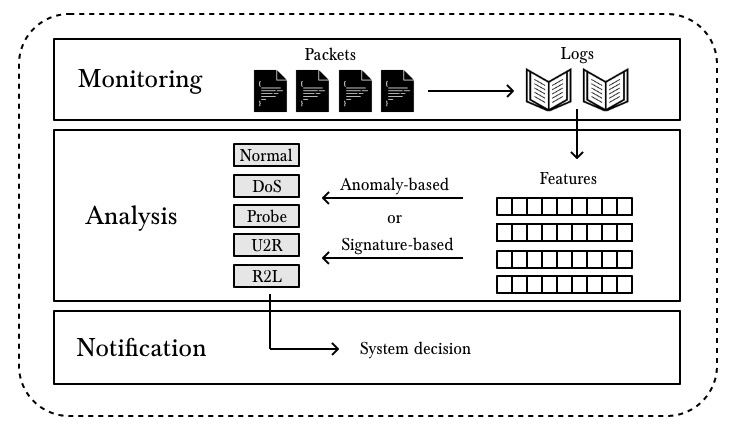
\includegraphics[width=.95\textwidth]{parts/chap-2/img-2/ids-model.jpg}
    \caption[Structure of an intrusion detection system]{General structure of an intrusion detection system. The different attack classes are based here on chapter~\ref{cha:4}.} 
    \label{img:ids-model}
\end{figure}

\subsection{Extraction of features}
Packets to be analyzed have a huge size and cannot be analyzed as such by the IDS. They typically incorporate huge redundancy and other non-necessary information such as padding. The idea of feature reduction is to reduce the packets to a limited number of features, representing as much non-redundant information as possible. Examples of features extracted consist of the connection length, the protocol used, the number of bytes transferred from the source to the destination and vice-versa.


\subsection{Pattern analysis}
The goal of the analysis of the IDS is to categorize the packets into different classes, typically a normal class and some different attack classes. As stated in the introduction, this can be done by two different manners based on a signature (\emph{signature-based}) and using some statistical rules (\emph{anomaly-based}). In this thesis, we will interest us to anomaly-based IDS, more specifically using classification machine-learning algorithms. The goal is that a user is able to classify its (query) on external trained machine-learning algorithm from one or more other parties, called the model owner(s). Furthermore, these algorithms have to be privacy-friendly in the sense that nor the query, nor the information resulting from the training should be revealed. This chapter aims at describing the two main machine-learning algorithms used without any consideration of the privacy-friendliness that will be covered in chapter~\ref{cha:3}.

\FloatBarrier
\section{Data reduction}


\subsection{Instance set size reduction}
Instance-based learning algorithms are often faced with the problem of deciding which instances to store for use during generalization. Storing too many instances can result in large memory requirements and slow execution speed, and can cause an oversensitivity to noise. \noteH{Input size so big as possible to reduce variance of the results}

In the practice, the data can be classified into two kind of classes, attack and no attack, or normal. In a practical intrusion detection system, most of the traffic is normal and sole a few proportion is attacking. We thus want to reduce the size of the normal data-set to make it of a similar size to the attack classes. Furthermore, the normal instances are very diversified and one may not just reduce the set randomly in the risk of missing relevant instances. One must thus find a more intelligent heuristic to decide which normal instances to keep.

How to decide which instances keep?
Keep only the ones near to the decision boundary. (+ explain what is a decision boundary). Way of keeping the sole normal instances near the decision boundary out of a way bigger set and thus build a more relevant training set of normal instances.

\subsubsection{$k$-means clustering}
The $k$-means clustering algorithm is a semi-supervised instance set reduction algorithm. This a specific case of clustering methods, that aim to divide the original data-set into smaller $k$ smaller clusters that should share some common properties. The challenge here is to find the most homogeneous possible clusters, which instances are similar enough --- referred to as the minimisation of \emph{intra-class inertia} ---, but not too many so that the clusters are well differentiated -- also referred to as the maximiastion of \emph{inter-class intertia}. After this being achieved, one can thus reduce each cluster far from the decision boundary to an archetype instance of this cluster and keep the clusters near the decision boundary. The algorithm is semi-supervised as the clustering in itself is only based on the features set, but is only applied on the data-points that are classified as normal, which of course depends on the target space.

To determine the different clusters, the $k$-means algorithm tries to minimize the distance between the instances in each cluster $\mathcal{S}_i$. The number clusters is fixed to $k$, which an hyper-parameter of the model set by the user. Computing the distance between each of the points would require a quadratic at each evaluation of cluster. To keep the complexity linear, the distances are not computed between each of the instances, but between each of the instances and the mean of these instances $\mu_i = \left( \sum_{x_j \in \mathcal{S}_i} x_j\right)/\vert \mathcal{S}_i \vert$ where $\vert \mathcal{S}_i \vert$ is the number of instances in the cluster.
\begin{equation}
    \underset{\mathcal{S}}{\mathrm{arg}\,\mathrm{min}} \sum_{i=1}^k \sum_{x_i \in \mathcal{S}_i} \norm{x_j-\mu_i}^2
\end{equation}
Defining the optimal clusters would at least be exponentially complex in function of the number of total instances as each cluster combination would have to be tested. Therefore, the $k$-means algorithm starts with assigning the starting clusters to initial data-points, chosen at random in our case. It then goes through the whole data-set and assigns each point to the cluster with the nearest mean $\mu_i$. The means are then updated and the process starts again. This is given at algorithm~\ref{alg:k-means}. Although doesn't guarantees any optimality nor polynomial computational time, it is considered very effective in the practice \cite{Arthur2006Worst-caseMethod}.

\begin{center}
\begin{algorithm}[H]
 \KwData{Feature data-set $\mathcal{F} = \left\{x_i\right\}_{i=1 \ldots n}$ and number of cluster sets $k$}
 \KwResult{$k$ clusters $\mathcal{S}_i = \left\{x_i\right\}_{i=1 \ldots m_i}$}
\DontPrintSemicolon

\lForEach{i = 1\ldots k}{
$\mu_i \leftarrow$ random $x_j$
}
\Repeat{$\mathrm{convergence}$}{
\ForEach{$x_j \in \mathcal{F}$}{
\lForEach{$i = 1\ldots k$}{$d_{i} \leftarrow \norm{x_j-\mu_i}$ \;}
$l \leftarrow \mathrm{arg}\,\mathrm{min} d_i$ \;
assign $x_j$ to $\mathcal{S}_l$ \;
}
\ForEach{$i = 1\ldots k$}{
$\mu_i \leftarrow \mu_i = \frac{1}{\vert \mathcal{S}_i \vert}\left( \sum_{x_j \in \mathcal{S}_i} x_j\right)$
}
}
\Return{$\mathcal{S}_{1 \ldots k}$}
\caption{The $k$-means algorithm. The convergence criterion typically is no more evolution in the means or the composition of the clusters, which is almost always equivalent in the practice.}
\label{alg:k-means}
\end{algorithm}
\end{center}

Once the clusters are determined, we can remove the normal data instances of the farthest from the decision boundary and replace the whole cluster by its mean $\mu_i$. In this way, we reduce the number of points far from the decision boundary and keep all the ones near the decision boundary. The number of set to be reduced $p<k$ is also an hyper-parameter set by the user. A way to determine which one are the farthest is just to compute the distance between the mean of each cluster and the mean of the attack instances defined in the same way.

\subsection{Feature size reduction}
+ explain why reduce the feature size. Complexity gain and better suited for distance calculation. Avoid curse of dimensionality. Avoid participation of non-relevant features in the training of the classification algorithm.

\subsubsection{Principal components analysis}
A linear Principal Components Analysis dimensionality reduction consists in a spectral analysis of the covariance matrix $\mathbf{\hat{\Sigma}}$ \noteH{(+ give forula for covariance matrix)} which can diagonalized with nonnegative eigenvalues $\lambda_i$ as it is semi-positive definite
\begin{equation}
\hat{\Sigma}x = \lambda_ix
\end{equation}
The $M$ greatest eigenvalues are then kept and the data transformed accordingly:
\begin{equation}
z_i = x_i^Tx
\end{equation}
Here is an attempt of an intuitive understanding of the process. Each input variable of the original input vector is independent, but some have strong underlying relations between them, measured by their covariance matrix. By diagonalizing it, there result $n_f$ new variables without any linear underlying relation. In a certain way, the eigenvectors $x_j$ represent these relations and their respective eigenvalues $\lambda_j$ their contribution, thus their importance. We can then afford to drop the non-important ones.

In our case, each feature is first being normalized, i.e. zero mean and unit variance. In other words, the covariance matrix has an unit diagonal and with a feature dimension of $n_f$, we have $tr(\hat{\mathbf{\Sigma}})=n_f$ which corresponds in a certain way to the total variance of the whole feature space. Quite logically, the latter is invariant to any linear transformation as the trace is an invariant to any linear transformation. The main idea behind linear PCA analysis reduction is thus to keep the richness of the data a maximum, thus its total variance, and reducing its dimension a maximum by dropping its smallest contributors. A good measure for the relative importance of each eigenvector, or underlying linear relation, is its fraction or variance contribution given by
\begin{equation}
f_j = \lambda_j/\Sigma_{\forall j}\lambda_j = \lambda_j/\tr\left(\hat{\mathbf{\Sigma}}\right)
\end{equation}

One can then choose the input values it decides to keep in descending order of the respective fractions $f_j$.

\subsubsection{Kernel principal components analysis and Mercer's trick}
The main problem of PCA is that it limits to linear relations between the feature elements. However, feature relations, especially in high dimension spaces require non-linear relations. Therefore, it would be interesting to map the instances into a space of higher dimension $\phi(x)$.

Therefore, we may now compute the covariance matrix in the mapped space $\phi\left( \mathcal{F} \right)$ of the feature space $\mathcal{F}$
\begin{equation}
    \hat{\Sigma}_{\phi} = \frac{1}{n_f} \sum_{x_i,x_j \in \mathcal{F}} \left( \phi(x_i) - \mathrm{mean} \right) \cdot \left( \phi(x_j) - \mathrm{mean} \right)
\end{equation}

Fortunately, there exists a method to compute this easily. Mercer's trick \cite{Minh2006MercersSmoothing}, also known as \emph{the kernel trick} can be used when an algorithm is based on the sole scalar product between feature vectors instances. It can then be replaced by a \emph{kernel matrix} representing the scalar product of the transformations.
\begin{equation}
    K_{ij} = K(x_i,x_j) = \phi(x_i) \cdot \phi(x_j)
\end{equation}

To compute the covariance matrix, we first have to centralize the data, which can be easily done with simple matrices multiplication
\begin{eqnarray}
    K_{ij}'&=& K_{ij} - \frac{2}{n_f} \sum_k^{n_f}\left( K_{ik}+K_{jk} \right) + \frac{1}{n_f^2} \sum_{l,m,n,o}^{n_f}K_{lm}K_{no} \\
    K' &=& K - 1_{n_f}K - K1_{n_f}+ 1_{n_f}K1_{n_f}
\end{eqnarray}
where $1_{n_f}$ represents matrices of the size $\left( n_f , n_f \right)$ where all elements are equal to $1/n_f$.

We can now perform a diagonalization on this new covariance matrix of the transformed data-points and perform the classification on them. This method is called \emph{kernel principal components analysis} (KPCA). 

A very interesting property of the kernel matrix is there is no need for computing the explicit transformation of each data-point as we are only interested in their scalar product. Indeed, they are never used on their own, but always in the kernel matrix. As such, one may directly compute the direct matrix. This is even more interesting as the scalar product of most of the transformations are mapped into an infinite dimension feature space and the scalar product can only theoretically be computed in Hilbert sace. Different kernel functions are possible, that represent the scalar product of different transformations. These kernel functions rely more often on one or more hyper-parameter that has to be trained. The most common choices are
\begin{itemize}
    \item \textbf{Linear kernel function:} this corresponds to computing directly the scalar product onto the identity transformation $\phi(x_i)=x_i$ and is thus equivalent to a linear PCA analysis.
    \begin{equation}
        K(x_i,x_j) = x_i \cdot x_j
    \end{equation}
    \item \textbf{Radial basis function kernel function (RBF):} this kernel function has one hyper-parameter. At a scale factor excepted \noteH{(à une constante près ?)}, this corresponds to the probability of the second instance given the first one with standard deviation $\sigma$. An interesting property of this kernel function is its ability to measure similarity as it converges to zero as the distance between both data-points increase and the point thus becoming more and more dissimilar. RBF are known to have excellent generalization capabilities.
    \begin{equation}
        K(x_i,x_j) = e^{\frac{-\norm{x_i-x_j}^2}{2\sigma^2}}
    \end{equation}
    \item \textbf{Polynomial kernel function:} this kernel function also has one hyper-parameter $d$. In the practice, $d=2$ is often chosen as higher order tend to overfit.
    \begin{equation}
        K(x_i,x_j) = (x_i \cdot x_j +1)^d
    \end{equation}
\end{itemize}

Due to their strong generalization power, RBF kernel generally perform better than other kernels, especially if no additional knowledge of the data is available or multiclass problems as the different classes often are often more diverse and require more generalization. In the case of intrusion detection systems, RBF kernel functions also tend to show better results \cite{Kuang2014ADetection}. Though, other kernels seem to show better results in some specific binary cases \cite{Elkhadir2016IntrusionMethods}. In our case and as we will work with multi-class classifiers, we will also opt for RBF kernel functions.

\subsubsection{Chi-square feature selection}
Up to new, the idea was to reduce the feature size by constructing new ones as transformations of the original feature vectors. However, one also choose to to select a number of features and just not care about the other ones. Another interesting property would be to be able to reduce the feature size in a supervised way, taking the machine learning algorithm into account. This can be tackled with $\chi^2$-feature reduction.

This feature selection method is based on the $\chi^2$ statistical hypothesis test that measures the dependence of two variables.





$\chi^2$-feature reduction test have successfully been applied to some machine learning algorithms for intrusion detection systems and seem to deliver better results than PCA or KPCA \cite{SumaiyaThaseen2017IntrusionSVM}.
\section{Support Vector Machines}
Support vector machines are a set of supervised machine learning algorithms than can be used either for classification or regression proposed by Vapnik in 1963 \cite{VapLer63}. The main idea originates with binary classification and consists of finding an optimal hyper-plane between the data-points separating both target classes.

\subsection{Linear support vector machines}
In its primal form, the support vector machine corresponds to the following minimization problem
\begin{equation}
    \begin{aligned}
& \underset{x}{\text{minimize}} 
& & \frac{1}{2}w^Tw + C \sum_{k=1}^N \xi_k \\
& \text{subject to}
& & y_i\left[ w \cdot x_i+b \right] \geq 1-\xi_i, \; i = 1, \ldots, N \\
& 
& & \xi_i \geq 0, \; i = 1, \ldots, N.
\end{aligned}
\end{equation}
This corresponds to finding a hyper-plane defined by the vector $w$ and intercept $b$ that separates all the data-points. The minimization of $w^Tw = \norm{w}^2$ corresponds to maximizing the margin between the hyper-plane and the nearest data-points. This is the criterion used to define an unique hyper-plane as an infinity that separates the data-points correctly may exist. Indeed, the nearest data-points $x$ are on the parallel hyper-plane $w^Tx-b= \pm 1$. The distance between the margin and the nearest point is thus $1/\norm{w}$. Maximizing it means minimizing $\norm{w}$ and due to the monotony of the norm $\norm{w}^2 = w^Tw$.

Of course, it can happen that no hyper-plane is able to classify all points correctly. Slack variables $\xi_k$ are therefore introduced. The trade-off between the best possible classification of the data-points (the contribution of the slack variables) and the maximizing of the margin is controlled by the box contraint parameter $C$.

New data-points (queries) are estimated as
\begin{equation}
    \mathtt{SVM}(x) = w \cdot x + b 
\end{equation}
The classification is given by the side of the hyper-plane on which the data-point resides which corresponds to taking the sign of this estimation.

In comparison to other machine learning algorithms like neural networks for example, the SVMs present the big advantage taking the form of a convex optimization problem. But their greatest strength in my opinion is the ability to use transformations for representing a non-linear separation. Therefore, we have to to work in the dual space, where the SVM optimization problem now reformulates
\begin{equation}
    \begin{aligned}
& \underset{\alpha_i}{\text{maximize}} 
& & \sum_{i=1}^N \alpha_i - \frac12 \sum_{i,j=1}^N \alpha_i \alpha_j y_i y_j (x_i \cdot x_j) \\
& \text{subject to}
& & 0 \leq \alpha_i \leq C \; i = 1, \ldots, N \\
& 
& & \sum_{i=1}^N\alpha_i y_i = 0.
\end{aligned}
\end{equation}
and the estimation of a new data-point now becomes
\begin{equation}
    \mathtt{SVM}(x) = \sum_{i=1}^N \alpha_i y_i (x_i \cdot x) + b
\end{equation}
The dual formulation gives its name to support vector machines. A new data-point is estimated based on the other vectors from the training size and their corresponding weights. The box constraint parameter here corresponds to the maximum weight of a support vector. In the case of privacy-friendliness, support vectors are very sensitive data as they directly represent instances from the original training data-set.

\subsection{Mercer's trick and non-linear support vector machines}
The main problem of support vector machines as described above is that they are limited to linear relations between the feature elements. However, feature relations, especially in high dimension spaces require non-linear relations. Therefore, it would be interesting to map the instances into a space of higher dimension $\phi(x)$.

The feature vectors are only appearing in the form of a scalar product, which allows us to use Mercer's trick. The idea is to replace the scalar products by a kernel function $K(x_i,x_j) = \phi(x_i) \cdot \phi(x_j)$. In most kernel functions, the feature vector is mapped into a space of infinite dimension. We thereby have to consider the scalar product in a Hilbert space to keep the mathematical sense of it: $\phi(x_i) \cdot \phi(x_j) = \langle \phi(x_i), \phi(x_j) \rangle_{\mathcal{H}}$.

We can define the kernel matrix as $K_{ij} = K(x_i,x_j)$. A very interesting property of the kernel matrix is there is no need for computing the explicit transformation of each data-point as we are only interested in their scalar product. Indeed, they are never used on their own, but always in the kernel matrix. As such, one may directly compute the direct matrix. This is even more interesting as the scalar product in Hilbert spaces are practically infeasible as such. Different kernel functions are possible, that represent the scalar product of different transformations. These kernel functions rely more often on one or more hyper-parameter that has to be trained. The most common choices are
\begin{itemize}
    \item \textbf{Linear kernel function:} this corresponds to computing directly the scalar product onto the identity transformation $\phi(x_i)=x_i$ and is thus equivalent to a linear PCA analysis.
    \begin{equation}
        K(x_i,x_j) = x_i \cdot x_j
    \end{equation}
    \item \textbf{Radial basis function kernel function (RBF):} this kernel function has one hyper-parameter. At a scale factor excepted, this corresponds to the probability of the second instance given the first one with standard deviation $\sigma$. An interesting property of this kernel function is its ability to measure similarity as it converges to zero as the distance between both data-points increase and the point thus becoming more and more dissimilar. RBF are known to have excellent generalization capabilities.
    \begin{equation}
        K(x_i,x_j) = e^{\frac{-\norm{x_i-x_j}^2}{2\sigma^2}}
    \end{equation}
    \item \textbf{Polynomial kernel function:} this kernel function also has one hyper-parameter $d$. In the practice, $d=2$ is often chosen as higher order tend to overfit.
    \begin{equation}
        K(x_i,x_j) = (x_i \cdot x_j +1)^d
    \end{equation}
\end{itemize}

Due to their strong generalization power, RBF kernel generally perform better than other kernels, especially if no additional knowledge of the data is available or multi-class problems as the different classes often are often more diverse and require more generalization. In the case of intrusion detection systems, RBF kernel functions also tend to show better results \cite{Kuang2014ADetection}. Though, other kernels seem to show better results in some specific binary cases \cite{Elkhadir2016IntrusionMethods}. In our case and as we will work with multi-class classifiers, we will also opt for RBF kernel functions.

The SVM dual formulation now becomes
\begin{equation}
    \begin{aligned}
& \underset{\alpha_i}{\text{maximize}} 
& & \sum_{i=1}^N \alpha_i - \frac12 \sum_{i,j=1}^N \alpha_i \alpha_j y_i y_j K(x_i, x_j) \\
& \text{subject to}
& & 0 \leq \alpha_i \leq C \; i = 1, \ldots, N \\
& 
& & \sum_{i=1}^N\alpha_i y_i = 0.
\end{aligned}
\end{equation}
with estimation
\begin{equation}
    \mathtt{SVM}(x) = \sum_{i=1}^N \alpha_i y_i K(x_i,x) + b
\end{equation}
However, there is also a downside: we are now facing an optimization problem in the dimension of the number of input instances and not of the dimension of the feature space anymore. This means that the number of support vector will drastically increase, which is a bad scenario for our privacy-friendly models. This is one of the investigated trade-offs.


\subsection{Multi-class SVMs}
The main problem of SVM for multi-class classification is that they are not natively suited for it. Indeed, SVM return a single number representing how far the tested data-point is from the hyper-plane. SVMs are by definition created for binary classification as the whole idea behind it is to separate the feature space into two parts. The kernel trick doesn't change anything to that as it only projects the data-point into a space of higher --- often unlimited --- dimension where a new hyper-plane is searched for, but still dividing this new higher dimension space into two parts.

Ideas for classifying SVMs into different classes could be for example to put the output number into bins. However, this is a very bad idea as it would in fact suggest that all the different classes are divided by parallel hyper-planes at a distances corresponding the the range of the bins, which range could also be trained (figure~\ref{mach:svm-model-gr-1}). It almost never occurs that one hyper-plane separates two classes perfectly, the fact that $n-1$ parallel hyper-planes separate the feature space according the the $n$ different classes is even less likely. This hypothesis is much too strong and must be discarded. We therefore have to use more than one SVM and combine them.

We will present here two different ways of combining SVMs that have both been tested in the case of intrusion detection systems \cite{Kuang2014ADetection}\cite{SumaiyaThaseen2017IntrusionSVM} and produce fairly similar results although they never have been compared using exactly the same model for the rest.

The first way and the most frequent one is to create $n$ different classifiers, each for a class, and to look at which one produces the best results. 
\begin{equation}
    \underset{k}{\mathrm{arg}\,\mathrm{min}}\left\{ \mathtt{SVM}_k (x_i)   \right\}_{1 \ldots n} 
\end{equation}
where $\mathtt{SVM}_k$ represents the SVM for each class $k$. Each classifier takes as binary input, +1 for the class and -1 for all the rest data-points  (figure~\ref{mach:svm-model-1}). A way of interpreting it is looking for which SVM the data-point lies the farthest from the hyper-plane, at its good size (i.e. positive). This can be graphically observed at figure~\ref{mach:svm-model-gr-2}. This is called the \emph{one-against-all} model.

\begin{figure}[ht!]
    \centering
    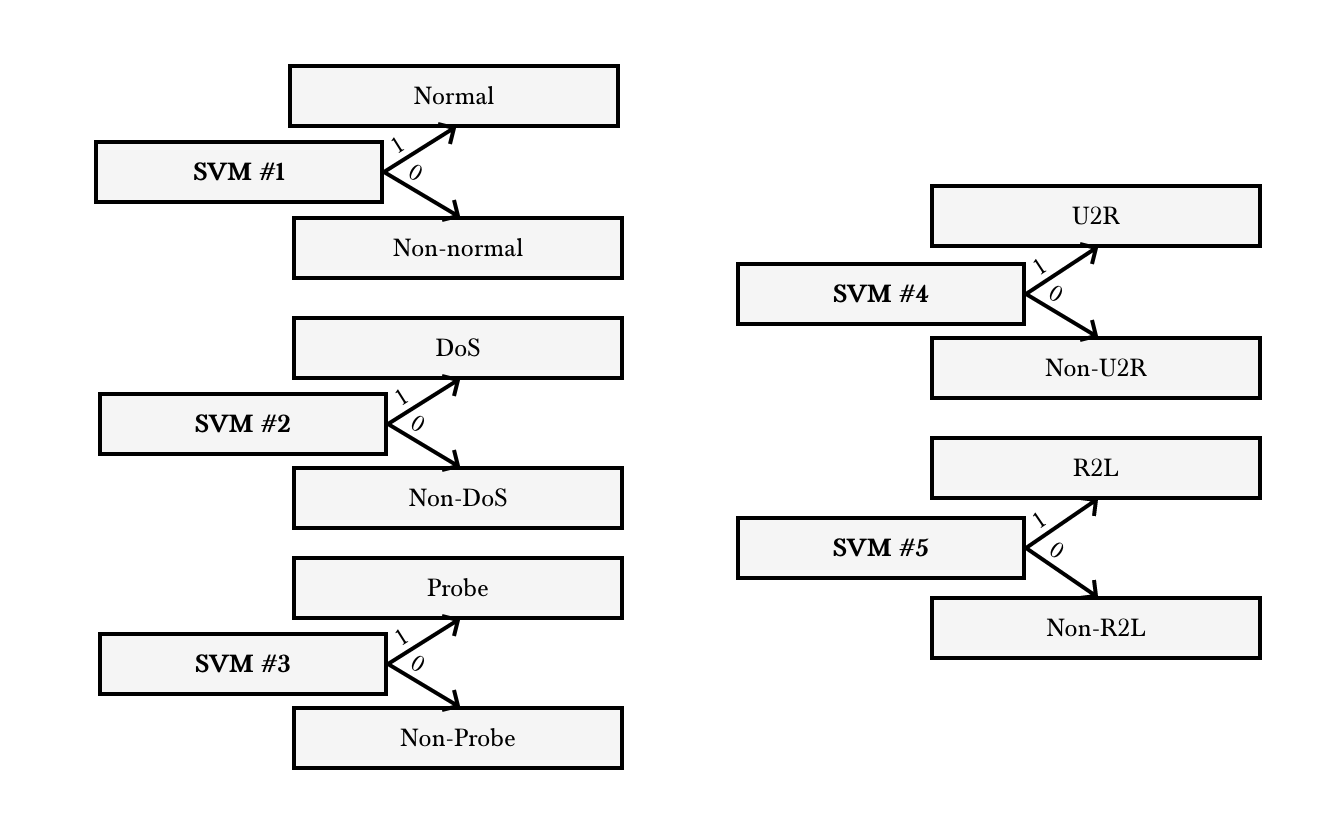
\includegraphics[width=.85\textwidth]{parts/chap-2/img-2/model-svm-1.png}
    \caption{One-against-all multi-class SVM model.} 
    \label{mach:svm-model-1}
\end{figure}

Another way of doing it is to work with successive SVMs as in figure~\ref{mach:svm-model-2} and is referred to as \emph{tree-based} models in this thesis. The first SVM is trained using one class as input versus all the others, as the first model. However the next classes are trained using one of the remaining classes versus the others remaining classes. The big advantage is that is only need $n-1$ different SVMs, which is one less compared to the previous model. Another advantage is that the last SVMs are trained one more specific data. However, the drawback is -- which is recurrent in series model --- that if one of the SVM isn't efficient, all the model is suffering. Graphically, this can be interpreted as first dividing the space with an hyper plane into two parts. One of the two parts is the subdivided into two new parts and so on (figure~\ref{mach:svm-model-gr-3}). Other tree structures are also to be considered, but this is not the scope of this thesis. We will limit ourselves to the consideration of these tree-structures in different orders. The goal of the machine-learning study of this thesis is to try to reduce the number of operations made by the evaluation of a query on the machine-learning algorithm. Computing 4 SVMs instead of 5 indeed decreases these number of computations. We thus want to investigate if this has an impact on the classification performance. A study on the comparison between the different tree-based models is a totally other subject which is not pursued here. We just limit ourselves to the different models found in the papers.

For the sake of completion, we also have to mention the existence of \emph{one-against-one} models where a binary classifier is trained for all combinations of two classes. The winning class it the one whose corresponding classifiers have the most positive outputs. However, this model needs $n_c(n_c-1)/2$ different classifiers where $n_c$ is the total number of classes, which is the opposite of the goal we are seeking.


\begin{figure}[ht!]
    \centering
    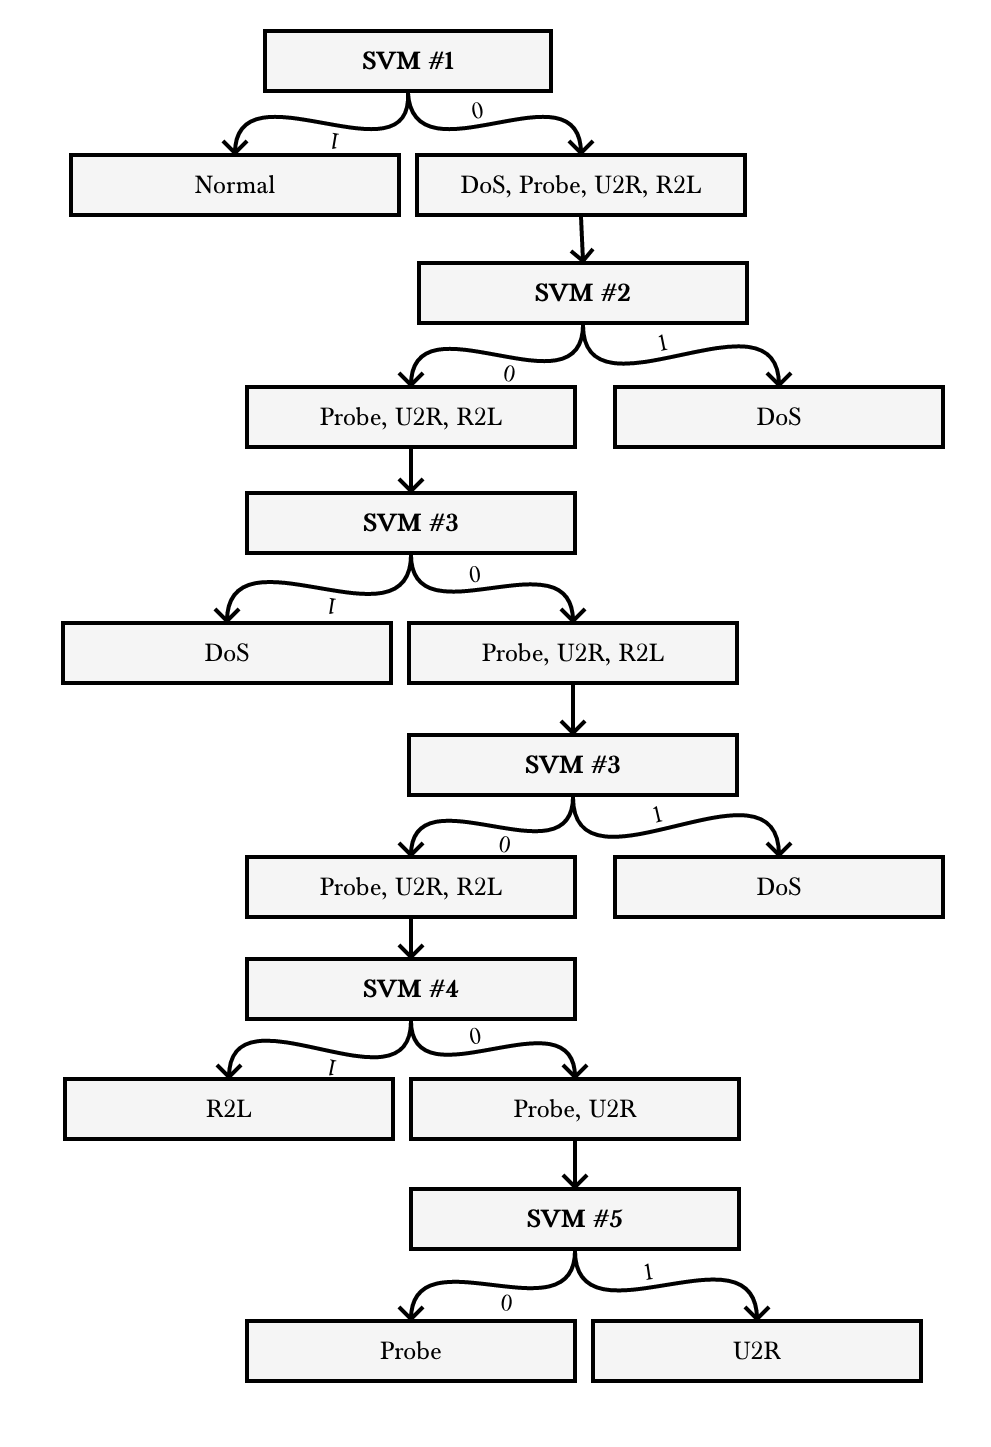
\includegraphics[width=.75\textwidth]{parts/chap-2/img-2/model-svm-2.png}
    \caption{Tree-based multi-class SVM model.} 
    \label{mach:svm-model-2}
\end{figure}

\begin{figure}
\begin{subfigure}[b]{0.32\textwidth}  
            \centering 
            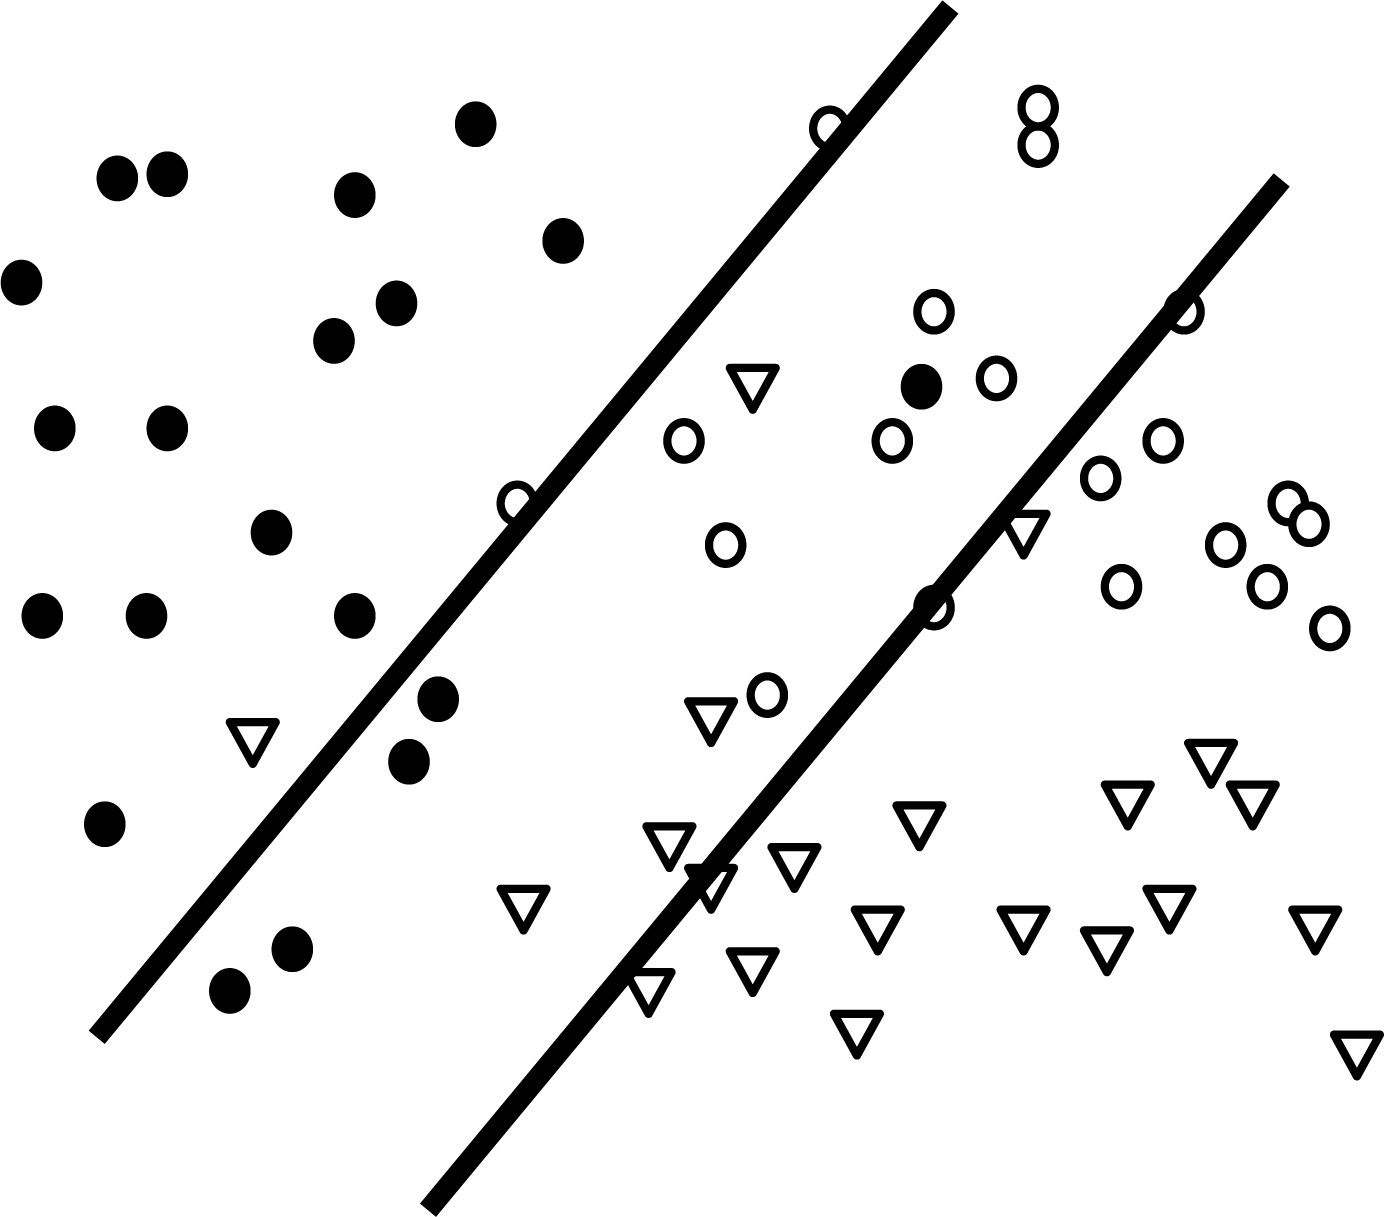
\includegraphics[width=.85\textwidth]{parts/chap-2/img-2/svm-par.png}
            \caption{Single SVM with bins.} 
            \label{mach:svm-model-gr-1}
        \end{subfigure}
        \hfill
        \begin{subfigure}[b]{0.32\textwidth}  
            \centering 
            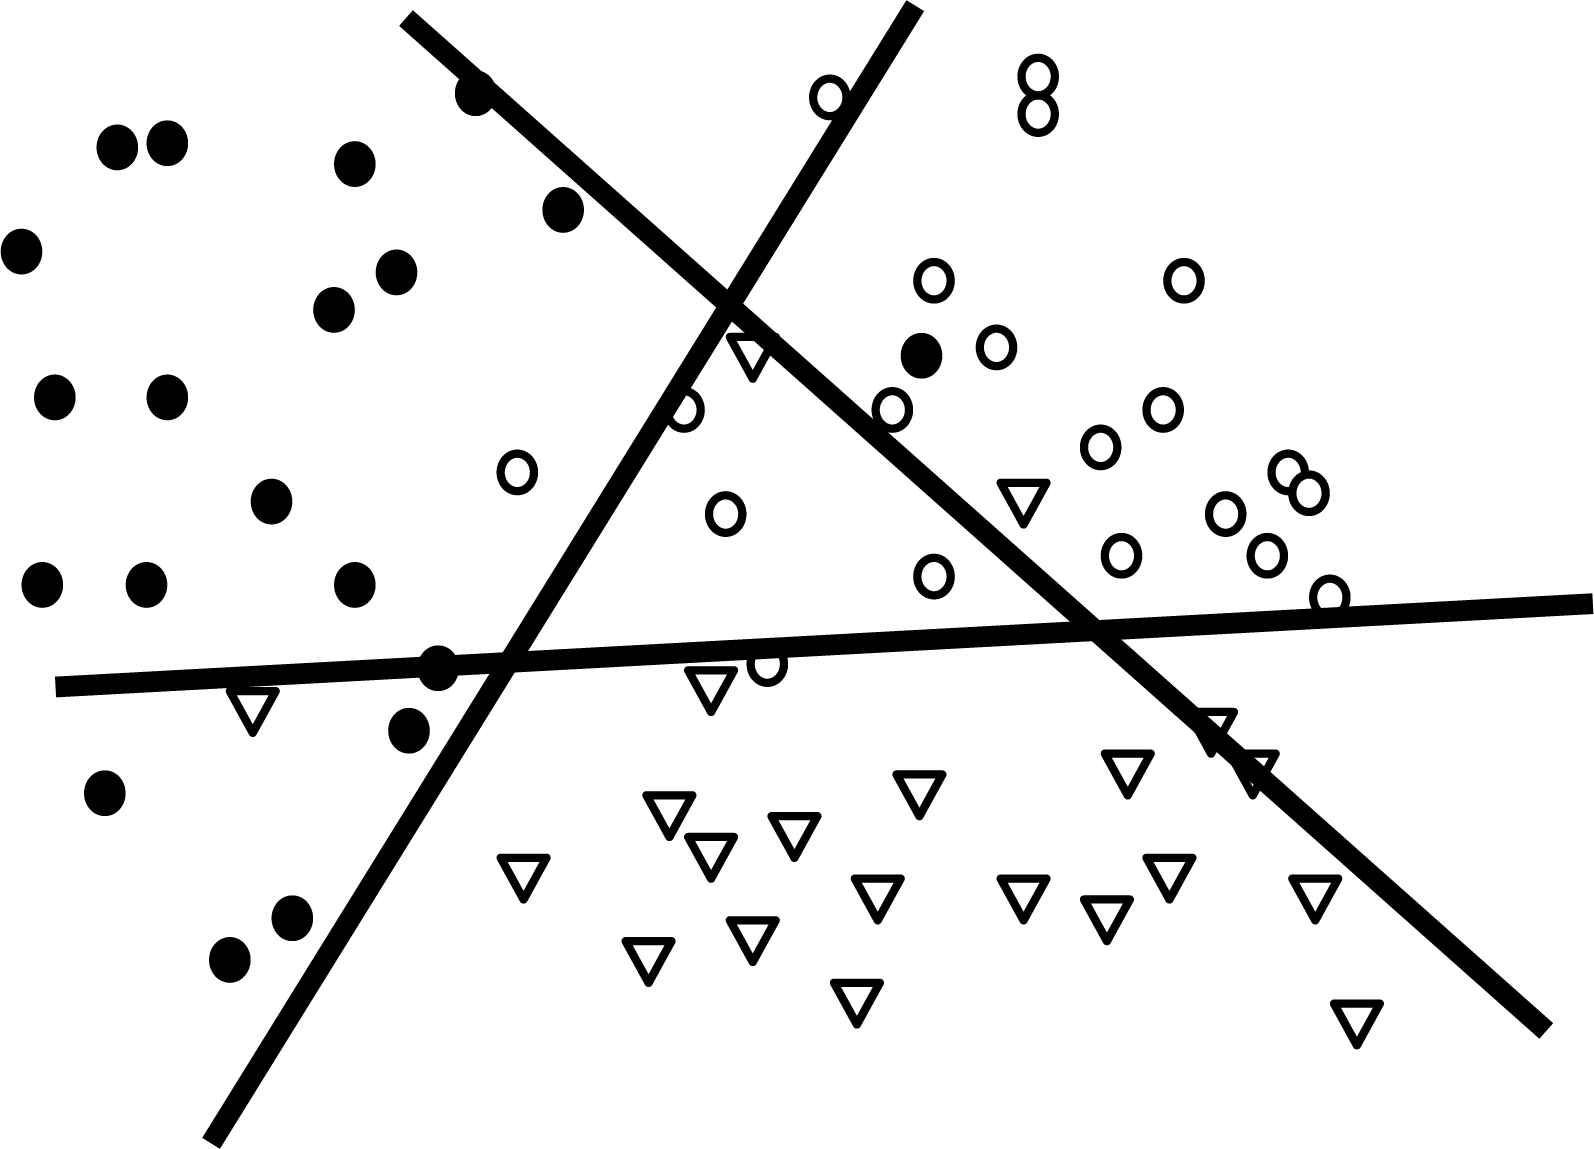
\includegraphics[width=.98\textwidth]{parts/chap-2/img-2/svm-multi.png}
            \caption{$n$ SVMs in a one-against-all model.} 
            \label{mach:svm-model-gr-2}
        \end{subfigure}
        \hfill
        \begin{subfigure}[b]{0.32\textwidth}   
            \centering 
            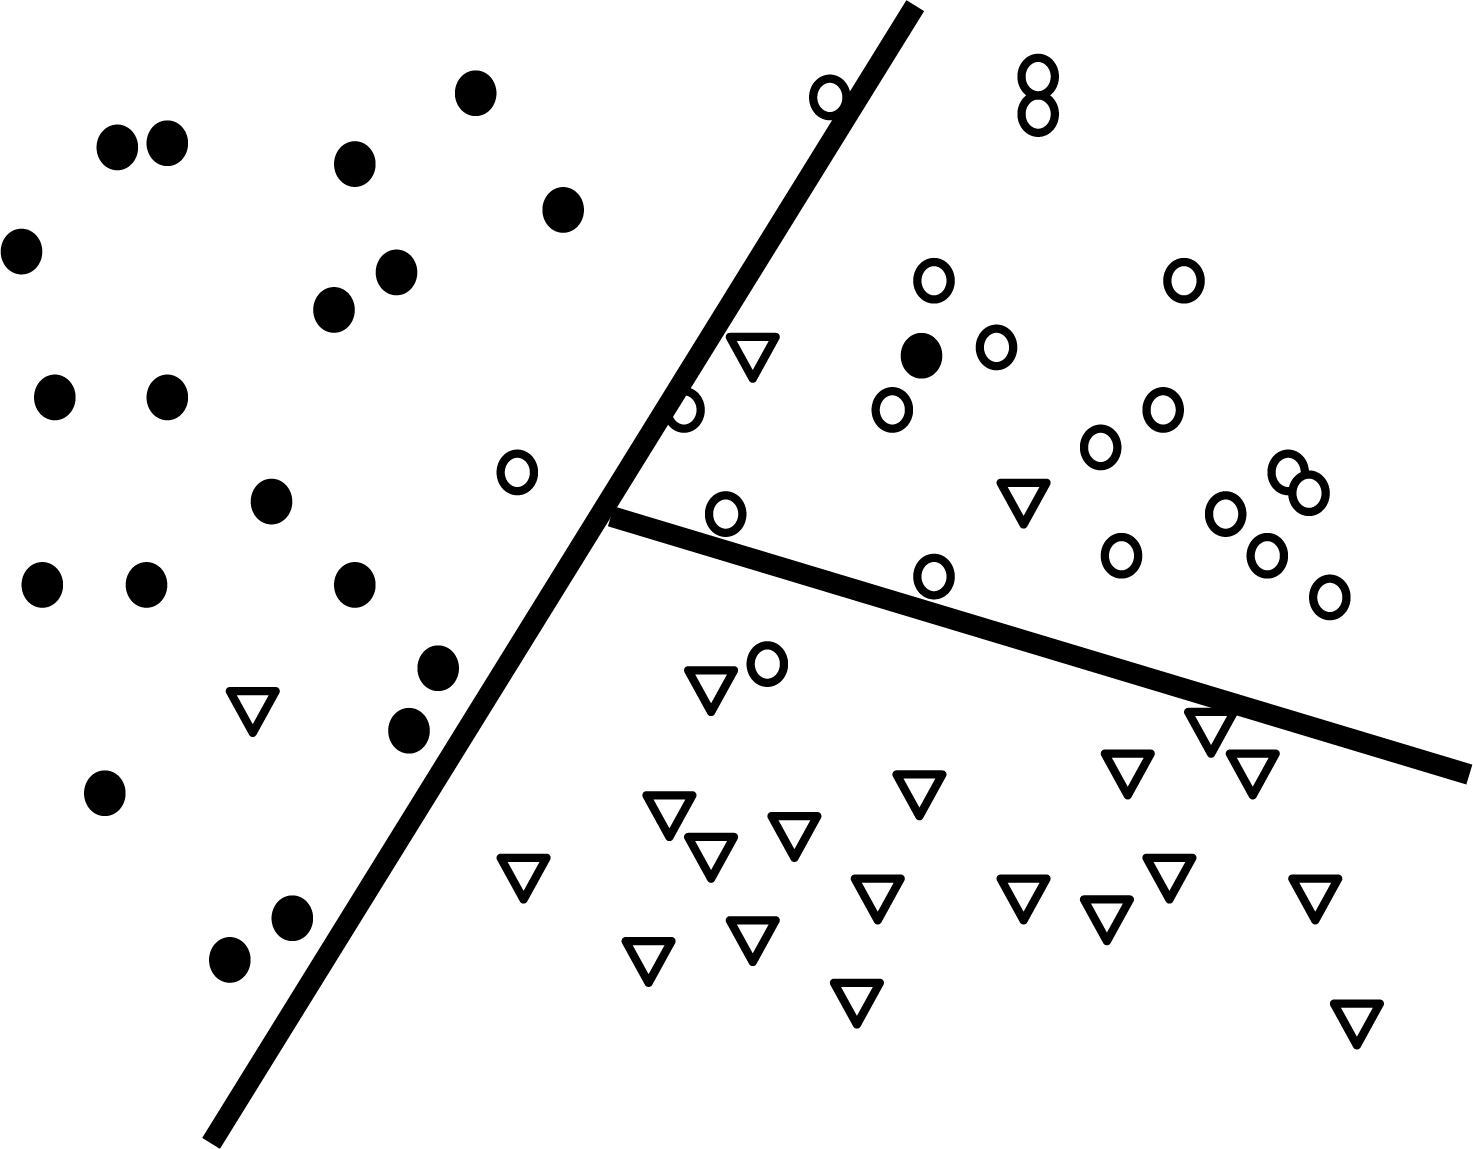
\includegraphics[width=.98\textwidth]{parts/chap-2/img-2/svm-seq.png}
            \caption{$n-1$ SVMs in a tree-based model.} 
            \label{mach:svm-model-gr-3}
        \end{subfigure}
        \caption{Comparison of different multi-class models in the feature space. In this case, there are three classes $n=3$: dots, circles and triangles.}
\end{figure}
\section{Nearest neighbour}
A classification algorithm that is often used in intrusion detection systems is the $k$-nearest neighbour ($k$-NN). This is a simple and effective method based on the distance of the elements in the feature space. Intuitively, when we want to characterize new data elements, we compare it to existent data elements and try to assign to it the characteristics --- in this case, the intrusion target --- of the similar ones. In other words, the test set elements are classified as similar training elements. Though, how do we count to elements to be similar, how do we measure similarity? In the $k$-NN algorithm, the elements are considered as data-points in the feature space and the similarity is measured as the euclidean distance between them. The most common target of the similar elements is then assigned to the test element.

More concretely, let's first consider a binary classifier of observations and targets $\left( x_1, y_1 \right), \ldots , \left( x_n, y_n \right)$ where observations $x_i \in \mathbb{R}^d$ and targets $y_i \in \left\{0,1\right\}$. To classify a new observation $\left( x_i, y_i \right)$, one just have to compare it to the $k$ other nearest observations and assign to the test observation the dominant target among its $k$ neighbours. In the classical $k$-NN algorithm, the neighbours are defined by the Euclidean distance. However, because of the monotony of the square function, one may use the square of the distances instead, avoiding to compute an extra square root, which is very useful in frameworks where operations are expensive like MPCs:
\begin{equation}
    \mathrm{d}^2\left( x_i, x_j \right) = \norm{x_i-x_j}^2 = \sum_{k=1}^d \left( x_{ik}, x_{jk} \right)^2
\end{equation}

Unlike binary classification algorithms like SVMs, $k$-NN algorithms are suited for multi-class problems without requiring any construction. However, they have also been used for binary classification in a construction \cite{Aburomman2016ASystem}. 

\subsection{Condensed Nearest Neighbours Data Reduction}
The problem of the nearest neighbours algorithm is its time to compute for large database. First, the computation of the distances increases linearly with the number of training points for each test points, thus quadratically if the number the test set has the same size as the training set. Secondly, the finding of the nearest neighbours takes requires O(kn) datapoints ... As we will see, one of the main trade-offs of MPC is the drastic increase in execution time. Therefore, the reduction of data-points becomes a necessity for the use of MPC-based $k$-NN.

The \emph{condensed nearest neighbours data reduction} (CNN) algorithm aims at finding the sole relevant data-points in the whole training set. The unclassified data-points then only need to be compared with the prototype points and not the whole database anymore. It is based on the idea that misclassified data-points lie close to the decision boundary, and one can just keep the data-points near the decision boundary and discard the others. The goal of the algorithm is to classify all training data-points into three categories:
\begin{itemize}
    \item \textbf{Outliers:} points which would not be recognized as the correct type if added to the database later. In other words, these data-points are the ones making the model perform worse with them than without. They increase the complexity of the decision boundary and increase significantly the number of kepts data-points and thus the relevance of the algorithm as it tries to keep a minimum of points defining the decision boundary. These points are to be discarded.
    \item \textbf{Prototypes:} the minimum set of points required in the training set for all the other non-outlier points to be correctly recognized. These data-points thus contain almost all of the relevant data. These points define the decision boundary and are to be kept.
    \item \textbf{Absorbed points:} points which are not outliers, and would be correctly recognized based on the sole prototype points. This could also be characterized as the redundant data. These points are far from the decision boundary and are to be discarded.
\end{itemize}

The outliers are first found by testing all existing points against the rest of the database with the chosen number $k$ of neighbours. If the point isn't recognized as the correct class, it is considered as an outlier, otherwise not. After defining all the outliers, one can proceed into the classification the restant data-points as prototypes or absorbed points. This is done in the next manner. Each point is once again tested against the dataset without the outliers, but with one sole neighbour, i.e. $k=1$. If it is well classified, it is considered as an absorbed point and can be left out of the final dataset. Otherwise, it is considered as a prototype ans is considered relevant to the classification or not redundant. These data-points are the sole ones making it to the final dataset. All points are tested until no prototype anymore makes it into the final dataset. The CNN data-reduction is given at algorithm~\ref{alg:cnn}.

In the condensed nearest neighbours algorithm, all new data-points are tested against the reduced database. Another big advantage of this algorithm is that the algorithm now always has to be used with $k=1$ because of the way we defined our prototypes and the final algorithm is thus faster. However, the classification with CNN will most of the time lead to a slightly different classification than with the classical $k$-NN against the whole dataset. Let's now investigate the classification trade-off in the case of our intrusion detection system database. 

\begin{center}
\begin{algorithm}[H]
 \KwData{Set $\mathcal{S}$ of $n$ feature points $\left\{x_i\right\}_{i=1 \ldots n}$ and corresponding targets $\left\{y_i\right\}_{i=1 \ldots n}$, number of neighbours $k$ for outlier detection}
 \KwResult{Reduced set $\mathcal{R}$ of $m<n$ feature points $\left\{x_i\right\}_{i=1 \ldots m}$ and corresponding targets $\left\{y_i\right\}_{i=1 \ldots m}$}
\DontPrintSemicolon
\SetKwFunction{FkNN}{kNN}

\ForEach{$\left(x_i, y_i\right) \in \mathcal{S}$}{
$t \leftarrow $\FkNN{$k$, $x_i$, $\mathcal{S}$} \;
\lIf{$t \neq y_i$}{remove chosen $\left(x_i, y_i\right)$ from $\mathcal{S}$}
}
$\mathcal{R}_0 \leftarrow \emptyset$ \;
add random $\left(x_i, y_i\right)$ to $\mathcal{S}$ \;

\Repeat{$\mathcal{R}_0 = \mathcal{R}_1$}{
$\mathcal{R}_1 \leftarrow \mathcal{R}_0$ \;
\For{$\left(x_i, y_i\right) \in \mathcal{S}$}{
$s \leftarrow $\FkNN{$k=1$, $x_i$, $\mathcal{R}_1$} \;
\lIf{$s \neq y_i$}{add $\left(x_i, y_i\right)$ to $\mathcal{R}_1$}
}
}
\Return{$\mathcal{R}_1$}
\caption{The condensed nearest neighbours algorithm. This algorithm relies on an implementation of the $k$-NN, represented here by the $\mathtt{kNN}$ function that takes as input the number of neighbours $k$, the data-points to be classified $x_i$ and the set in which it should search for the neighbours $\mathcal{S}$.}
\label{alg:cnn}
\end{algorithm}
\end{center}
\section{Ensemble methods}
\subsection{Bagging}
Bagging, short for \emph{boostrap aggregating} has first been described by Breiman \cite{Breiman1996BaggingPredictors}. Instead of one instance of a model trained on a whole learning set, different instances are trained with different bootstrap replicates of the original learning set. The final inference is then made by a majority vote on the different results. In other words, this method averages the set of the different possible learned models and reduces the instability of the prediction method. 

Let's consider a data-set of $N$ elements $\mathcal{L}=\left\{ \left( x_n,y_n\right),n=1,...,N\right\}$ where $x$ is the input vector and $y$ the output vector. The idea is to minimise the variation of the predictor $\hat{y}=\phi\left(x,\mathcal{L}\right)$ by calculating its expectation over the distribution of $\mathcal{L}$
\begin{equation}
    \phi_A\left(x,\mathcal{L}\right) = \mathbb{E}_\mathcal{L} \phi\left(x,\mathcal{L}\right) \approx A \left( \left\{ \phi\left(x,\mathcal{L}_k\right) \right\} \right) \qquad k=1,\, \ldots,\, N_k
\end{equation}
where $A$ is an aggregation function (\emph{i.e.} mean for a regression or a majority vote for a classification) and $\mathcal{L}_k$ different instances of the distribution of $\mathcal{L}$. As the instances set $\{ \mathcal{L}_k \}$ is not available, a bootstrap set $\{\mathcal{L}^{(B)}\}$ is constructed, each instance consisting of $N$ elements drawn randomly from the original $\mathcal{L}$, but \emph{with replacement}. The average prediction is then calculated as
\begin{equation}
    \phi_B\left(x,\mathcal{L}\right) = A(\{ \phi(x,\mathcal{L}^{(B)}) \})
\end{equation}
In his experiments, Breiman noted that 25 a 50 bootstrap replicates $N_k$ seemed a reasonable choice. In a certain sense, one could see bagging as a variant of cross-validation method on the whole learning process: a sort of \emph{cross-learning} with replacement.

The reason why bagging works is the much lower mean-squared prediction error of $\phi_A$ compared to $\phi$. Nevertheless, the fact of using the available $\phi_B$ instead of the theoretical $\phi_A$ has also drawbacks as it can deteriorate the prediction of already stable classifiers. In other words, bagging unstable classifiers such as neural nets, classification and linear regressions, usually improves them, whereas bagging usually stable classifiers such as $k$-nearest neighbours is not a good idea \cite{Breiman1996HeuristicsSelection}.

\subsection{Influence of MPC}
Compare naïve bootstrapping (each bootstraps its own copy) and full bootstrapping as described above. Can be done in parallel (MPC wins a lot from parallelization).

\subsubsection{Boosting}
The boosting method is based on a proof by Schapire \cite{Schapire1989} that weak learnability, an algorithm that slightly out-performs a random classifier, is equivalent to a strong classifier. To prove this equivalence, he used an algorithm that sequentially trains classifiers. Each classifier has a training set consisting of half well-classified elements of the previous one and half of wrongly classified elements, the first classifier starting from the original training set. Based on this idea, a later algorithm, called \emph{adaptive boosting} was developed based on a better distribution of the missclassified elements for creating the subsequent training sets \cite{Freund1997ABoosting}. + majority vote from all classifiers.

+ intuitively the algorithm will perform better when learning from the more difficult elements. In a certain sense, the more complex elements will have more degrees of freedom (not sure of this one).
\chapter{Achieving the preservation of privacy}
\label{cha:3}

\section{Different approaches on privacy-friendliness}
In a world of constant data exchange between different entities, it might be useful to develop methods not only to protect data during the transit as described before, but also when in possession of an entity that should not be able to read all of it. This is of particular interest for computation outsourcing where a specific data-set has to be processed by an external entity that should not be able to infer anything more than what is asked from it. Furthermore, it might even be wished that one or more external entities might not be able to read the output of their computations, solely readable by the owner(s) of the data. This is of particular interest for the --- now everywhere --- cloud solutions. A protocol that respects the private character of data when treated by other entities than the owner is called \emph{privacy-friendly} or \emph{privacy-preserving}. There exists different approaches to privacy-friendliness and for the stake of completeness, hereafter follows a short survey of them which also justifies our choice.

\subsection{Differential privacy}
Instead of encrypting all the data, one could alternatively directly address the core problem of why we want them encrypted: to prevent other parties to get any information on what data we possess. In the case that will interest us in this thesis, we will be in possession of a lot of data from personal users which is confidential and can therefore not be traced back to the user. In 2009, Netflix launched the Netflix prize on data recommendation: the first group to improve their recommendation score by 10\% or more would win 1.000.000\$. They provided a data-set to let the participants train their models and took care of anonymising the data before they made it accessible. However, Narayanan and Shmatikov showed how they could re-identify a lot of the users using the scores of the users on IMDb. \emph{Differential privacy} \cite{Dwork2008DifferentialResults} addresses this problem by adding noise to the data and thereby achieving a better anonymisation. In this way, the data is still usable for statistical models but cannot be used to identify anyone as easily as before. Still, differential privacy is limited by the fundamental and intrinsic relation between anonymisation and statistical relevance. One cannot obtain the first without inevitably having an influence on the second one, and reciprocally.

\subsection{Homomorphic encryption}
Differential analysis is a statistical approach of anonymity, but there exists also some cryptographic approaches, where the external entity is not able to read the results of what it produces. It is possible to construct a protocol with one or more third parties in a way that they cannot possibly learn anything from what they are receiving nor what they are sending back: the information is processed in an encrypted and not a clear form. Encryption schemes that allow mathematical operations to be executed on the encrypted data are called \emph{homomorphic} and were first proposed by Rivest et al. in 1978. For example, the RSA encryption scheme preserves the multiplication over the encrypted data. The RSA encryption scheme is given by $\mathscr{E}(m)=m^e \mod N$. We thus have $\mathscr{E}(m_1) \cdot  \mathscr{E}(m_2) = \left(m_1^e \mod N \right)\left(m_2^e \mod N \right) = \left(m_1m_2\right)^e \mod N = \mathscr{E}(m_1m_2)$. Unfortunately, this property is only true for multiplication and is therefore quite limited in its applications. We therefore refer to RSA as a \emph{somewhat-homomorphic} encryption scheme (SHE). When all mathematical operations are possible, we say from the encryption scheme that it is \emph{fully-homomorphic} (FHE). Up to now, only some schemes based on finite fields possess this property. 

The most accomplished method up to now is called the \emph{Approximate Eigenvector Method} and is based on the \emph{Learning With Errors} (LWE) encryption scheme, which is also known for still being secure in a post-quantum era. If $C_1$ and $C_2$ are two matrices with common eigenvector $\vec{s}$, we notice that the sum or multiplication of their respective eigenvalues $m_1$ and $m_2$ corresponds to the eigenvalue of the sum or multiplication of $C_1$ and $C_2$ with respect to $\vec{s}$. The eigenvector act as a private key and the eigenvalues as the secrect messages. The scheme is thus fully homomorphic. However, eigenvectors are easy to find and the scheme is thus also insecure. To resolve this, the method uses approximate eigenvectors $\vec{s}C=m\vec{s}+\vec{e}\approx m\vec{s}$ which is known to be still solvable in finite fields under a few assumptions about the error $\vec{e}$.

\subsection{Multi-party computation}
When different parties participate to the input, the homomorphic encryption described above cannot be used anymore: all parties have to share the same secret key which makes their data still private with respect to the third party, but not to each other. Multi-party computation addresses this problem. Furthermore, it also allows the parties to compute a common function on their private inputs without needing one or more third parties. 

More concretely, let us now imagine a problem where the goal is to compute some common function $f$ over private inputs $x_i$. On other words we want to compute $f\left(x_1, \, \ldots, \, x_n\right) = \left( y_1, \, \ldots , \, y_n\right)$ where each input $x_i$ is privately provided by player $i$, which ultimately learns $y_i$ and nothing more: nor the other outputs, not the other inputs. A first naive implementation would be to trust a third party for privately receiving each player's input, computing the function and privately communicating the corresponding responses to everyone. However, it also possible to obtain the same results without the trust of a third party, where only the players are participating to the protocol. This is called \emph{multi-party computation} (MPC) also referred to as \emph{secure multi-party computation} (SMC). This approach has been chosen to solve our problem and will be now more extensively described in the next section.

Multi-party computation originated with the toy example presented by Yao in 1982 \cite{Yao1982ProtocolsComputations} and now known as the \emph{Millionaire's Problem}: two millionaires both want to know who is richer, but none of them want to disclose their fortune nor trust a third party. Other applications of MPC may concern electronic voting or solutions of private-data as a service (PDaaS).
The different methods defined hereunder have a common general way of working. The computation is done in rounds: each party computes its shares on its own and the exchanges the needed shares with other parties. The exchange do not happen in continuous but all together in what is called a round. A new computation phase can then take place followed by a next exchange phase.


\subsubsection{Bit-wise decomposition}
There basically exists two big family of multi-party computation protocols, each based on a different cryptographic primitive, which is the basic block or idea on which the whole protocol is based. The first one described here decomposes every operation into a boolean circuit and every value into its bits, hence its name. The cryptography takes place at bit-level.

\paragraph{Oblivious transfer}
The idea behind \emph{oblivious transfer} originally described by Rabin in 1981 \cite{Rabin1981HowTransfer.} is the transfer of an information in possession of a first party and asked by a second party without the first party knowing which information has been transferred. Hence, the name oblivious, or alternatively, unconscious. Different protocols exist and are all based on the \emph{RSA scheme}. 

The most common version is the \emph{1-2 oblivious transfer} \cite{Even1985AContracts} and goes as follows: Alice is in possession of two messages $m_0$ and $m_1$ and Bob wants to get message $m_p$. Alice first generates a set of private key $d$ and public key $(N,e)$ and sends two random messages $x_0$ and $x_1$ to Bob. He then generates a random message $k$ and encrypts it with the $x_i$ corresponding to the wanted message: $v = \left(x_p + k^e\right) \mod N$ and sends it to Alice. She then recovers both $k$ without knowing which one corresponds to Bob's original one: $k_i = \left(v-x_i^d\right) \mod N$. These $k_i$ then serve to encrypt the messages which are finally sent to Bob $s_i = m_i+k_i$. Bob can then only decrypt the wanted message $m_p = s_p-k$. 

This protocol has been generalised to more than two parties \cite{Ishai1997PrivateApplications,Shankar2008AlternativeTransfer,Tassa2011GeneralizedSharing}

\paragraph{Yao's garbled circuits}
\emph{Garbled circuits} (GC) were first introduced by Yao in 1986 \cite{Yao1986HowSecrets} and are now one of the most efficient solutions for generic secure two-party computation. A function has to be decomposed into a boolean circuit consisting of two-input gates (e.g. XOR and AND). Let's consider the simplest example of evaluating an AND-gate between Alice and Bob. Alice first generates a different random sequence --- also called \emph{labels} --- for each possible value of each input --- also called \emph{wires} --- and output. In the truth table, the output are then symmetrically encrypted with the hash of each corresponding input. These four resulting cyphertexts are then randomly permuted --- hence the name \emph{garbled} --- and sent to Bob. The garbling of an AND-gate is illustrated at table~\ref{tab:ang-garb}. Once Bob receives the garbled gate, he then asks Alice for her label. As they have been randomly chosen, she can send it to him without him possibly knowing what value it corresponds to. Afterwards, he also needs to know the label of his input. This part is a bit more tricky and is solved using the previously described \emph{oblivious transfer}. Bob can now compute the hash of the two labels and decrypt each element of the garbled gate until we find one corresponding with the garbled gate he received from Alice. He can then reveal the value to Alice either she can reveal the mapping of the garbling. The same principle can be used on a multi-gate circuit by garbling the sole end result.

\begin{figure}
        \begin{subfigure}[b]{.32\textwidth} 
            \centering 
            \begin{tabular}{IC{.6cm}|C{.6cm}IC{1.3cm}I}
            \hlineI
            A & B & output \\ \hlineI
            0 & 0 & 0  \\ \hline
            1 & 0 & 0 \\ \hline
            0 & 1 & 0 \\ \hline
            1 & 1 & 1 \\ \hlineI
            \end{tabular}
            \caption{Truth table.} 
        \end{subfigure}
        \hfill
        \begin{subfigure}[b]{.32\textwidth} 
            \centering 
            \begin{tabular}{IC{.6cm}|C{.6cm}IC{1.3cm}I}
            \hlineI
            A & B & output \\ \hlineI
            $x_A^0$ & $x_B^0$ & $x_{\textnormal{output}}^0$ \\ \hline
            $x_A^1$ & $x_B^0$ & $x_{\textnormal{output}}^0$ \\ \hline
            $x_A^0$ & $x_B^1$ & $x_{\textnormal{output}}^0$ \\ \hline
            $x_A^1$ & $x_B^1$ & $x_{\textnormal{output}}^1$ \\ \hlineI
            \end{tabular}
            \caption{Labelled truth table.} 
        \end{subfigure}
        \hfill
        \begin{subfigure}[b]{.32\textwidth}
            \centering 
            \begin{tabular}{IC{3.2cm}I}
            \hlineI
            output \\ \hlineI
            $\mathscr{E}_{H\left(x_A^1,x_B^0\right)}\left(x_{\textnormal{output}}^0\right)$ \\ \hline
            $\mathscr{E}_{H\left(x_A^1,x_B^1\right)}\left(x_{\textnormal{output}}^1\right)$ \\ \hline
            $\mathscr{E}_{H\left(x_A^0,x_B^0\right)}\left(x_{\textnormal{output}}^0\right)$ \\ \hline
            $\mathscr{E}_{H\left(x_A^0,x_B^1\right)}\left(x_{\textnormal{output}}^0\right)$ \\ \hlineI
            \end{tabular}
            \caption{Garbled output.} 
        \end{subfigure}
        \captionof{table}{Garbling of the AND-gate.}
        \label{tab:ang-garb}
\end{figure}

It is interesting to note that the secure evaluation of a sole AND-gate does not respect the principles of the multi-party computation, by definition of the AND-gate. Indeed, if the final solution is 1, both players know their respective input value, which is thus disclosed\footnote{This is not the case for the XOR-gate as an 1-output has two corresponding inputs possible, as has the 0-output}. Therefore, the total functions evaluated have to be totally surjective for each input. The circuit corresponding to the Millionaire's problem is given at figure~\ref{privacy:yao-comp} and while it consists of AND-gates, the function is totally subjective with respect to each millionaire's fortune.

\begin{figure}[ht!]
    \centering
    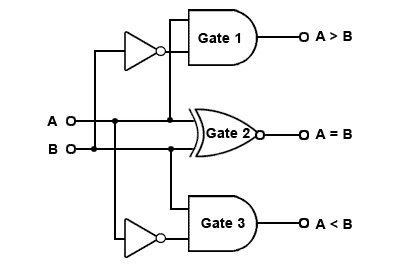
\includegraphics[width=.7\textwidth]{parts/chap-3/img-3/yao-comp.jpg}
    \caption{The figital comporator is the boolean circuit used to soleve Yao's millionnaire problem.} 
    \label{privacy:yao-comp}
\end{figure}

This protocol executes in polynomial time, but there exists a lots of optimisations that allow to garble and evaluate the gates more rapidly.

\paragraph{GMW protocol}
The \emph{Goldreich-Micali-Widgerson} (GMW) protocol can be seen as an extension of garbled circuits to multiple parties using Yao's idea of using oblivious transfer \cite{Goldreich1987HowGame}. The main principles here are based upon bit-sharing: each party shares its input bits among the $n$ players $b = \sum_{i=1\ldots n}b_i \mod 2$. Each player then processes their shares among the circuit. XOR-gates are easy as they can just addition the shares $c_i = a_i + b_i$. However AND-gates are more tricky: we can see from the decomposition that $c = a \cdot b = \sum_{i\neq j}a_ib_j+\sum_{1\leq i< j\neq n}\left(a_ib_j + a_jb_i \right) \mod 2$. By consequence, each party will have to compute $a_ib_i+ \sum_{i\neq j}\left( a_ib_j + a_jb_i\right)$. As for the XOR-gate, the first part is trivial to evaluate, however, the second cannot be computed by party $i$ without more information from party $j$. This is solved by using a variant of garbled circuits with oblivious transfer between parties $i$ and $j$.

\subsubsection{Avoiding bit-wise decomposition}
Alternatively, some arithmetic circuits can also be used for multi-party computation. The problem of the bit-wise decomposition and the use of the boolean circuit transcription of the function we jointly want to evaluate is their expensiveness in terms of performance. Indeed, a simple operation can rapidly lead to a lot of gates. For example, let's consider the addition of two number: for two numbers of $n$ bits, the total number of gates is $5n$ in a full adder composition. This is even worse for multiplication. Of course, some optimisations can be made, but the general number of gates is very high compared to the arithmetic circuit of the same function, where it would just be one single gate for addition and multiplication. We will see later that MPC over arithmetic circuits has a much higher \emph{round complexity} --- the dependence of the different rounds on each other --- which leads to less possible parallelisation than with boolean circuits. Nevertheless, one can argue that the parallelisation of bit-wise decomposition does not compensate the much higher number of gates and is thus less efficient than arithmetic circuits in general \cite{Aly2018PracticallyBit-Decomposition}. Even 2-party comparisons seem not so much more efficient with garbled circuits --- for which they were originally tailored -- compared to the method described hereunder \cite{Blom2014AThesis}.

The building block --- also called cryptographic primitive --- of multi-party computation over arithmetic circuits is based upon \emph{secret sharing}. Each party computes its own version of the circuit with the shares of the different parties. At the end of the circuit processing, each party has a share of the final output, which can then be put together to obtain the final output. We first have to define a way for a party to share its secret among $n$ parties, including itself.

\paragraph{Additive secret sharing}
The simplest idea is just to divide the secret $a$ in $n$ shares $a_i$ using a simple summation: $a = \sum_{i=1 \ldots n}a_i$. However, doing it in this manner allows the shares to release some information about the secret, as the shares are not random and strongly depend on the secret. They are two solutions to this problem and the first one is to consider additive sharing over $\mathbb{Z}_q$. The sharing now becomes $a = \sum_{i=1\ldots n}a_i \mod q$ which solves the problem, as the shares can now really be chosen at random. The other solution is over $\mathbb{Z}$ and consists in choosing a sufficiently large interval in which the shares are chosen to dilute sufficiently the statistical information about the secret, typically $a_i \in \left[-A2^\kappa,A2^\kappa\right]$ with $A$ the size of the interval of the secret $a \in \left[-A,A\right]$. The size of $a$ is of maximum bit-length $k$ and we therefore also refer to $\mathbb{Z}_k$ alternatively the interval.

Another consequence of this scheme is that all parties are vital to the recovery of secret as a loss of one secret unables us to reconstruct the secret or any statistical information about it as we took care of that. The scheme does not tolerate the loss or treason of one party and is therefore very sensitive to any failure or malicious player. This problem is solved by polynomial secret sharing.

\paragraph{Polynomial secret sharing}
The idea of polynomial sharing was originally proposed by Shamir in 1979 \cite{Shamir1979HowSecret}. This method allows $n$ parties to share a secret in a way such that any subset of $t+1$ parties can later reconstruct the secret but any subgroup of maximum $t$ parties cannot do so. The scheme is based on the single fact that for any polynomial of degree $d$, any subset of $d+1$ or more different points can reconstruct the polynomial completely whereas any subset of at most $d$ points is left with an infinite number of possibilities.

The scheme goes as follows. The party that wants to share its secret first constructs a polynomial of degree $t$.
\begin{equation}
    h(z) = a + \sum_{i=1}^t b_i z^i
\end{equation}
with secret $a$ random coefficients $b_i$. For the same reasons as for additive secret sharing, the coefficients can either be chosen in $b_i \in \mathbb{Z}_q$ (which also leads to the consideration of polynomial $h(z) \mod q$ instead), either in the interval $b_i \in \left[-A2^\kappa,A2^\kappa\right]$.
\noteH{should I demonstrate ?}

We verify that $h(0)=a$ and distribute shares $a_i$ to each party $i$ --- including ourselves --- as follows $a_i=h(i)$. $t+1$ parties can now reconstruct the polynomial together using e.g. Lagrange's polynomials and compute $f(0)$ to recover the secret share. An interesting property is that the recovery can be done as a simple linear combination. Indeed, we have
\begin{eqnarray}
    h(0) &=& \sum_{i=1}^{n} l_i(0)h(i) \\
    a &=& \sum_{i=1}^{n} r_ia_i
    \label{eqn:recover-secret}
\end{eqnarray}
where $r = \left(r_1, \ldots , r_n\right) = \left(l_1(0), \ldots , l_n(0)\right)$ is called the \emph{recombination vector} with $l_i(z)$ the $i$-th order Lagrange polynomial, for example
\begin{equation*}
    l_i(z) = \prod_{1\leq j \leq n,j\neq i}\frac{z-j}{i-j}
\end{equation*}
This also works with any generating set of $\mathbb{Z}\left[z\right]$ (or alternatively $\mathbb{Z}_q\left[z\right]$), as long all parties use the same set.
\section{Multi-party computation in a nutshell}
Multi-party computation originated with the toy example presented by Yao in 1982 \cite{Yao1982ProtocolsComputations} and now known as the \emph{Millionaire's Problem}: two millionaires both want to know who is richer, but none of them want to disclose their fortune nor trust a third party. Other applications of MPC may concern electronic voting or solutions of private-data as a service (PDaaS).

+ general description of rounds etc...

\subsection{Bit-wise decomposition}
Two types: bit-wise decomposition and additive sharing. Arithmetic and boolean circuits.

\subsubsection{Oblivious transfer}
The idea behind \emph{oblivious transfer} originally described by Rabin in 1981 \cite{Rabin1981HowTransfer.} is the transfer of an information in possession of a first party and asked by a second party without the first knowing which information has been transferred. Hence, the name oblivious, or alternatively, unconscious. Different protocols exist and are all based on the \emph{RSA scheme}. 

The most common version is the \emph{1-2 oblivious transfer} \cite{Even1985AContracts} and goes as follows: Alice is in possession of two messages $m_0$ and $m_1$ and Bob wants to get message $m_p$. Alice first generates a set of private key $d$ and public key $(N,e)$ and sends two random messages $x_0$ and $x_1$ to Bob. He then generates a random message $k$ and encrypts it with the $x_i$ corresponding to the wanted message: $v = \left(x_p + k^e\right) \mod N$ and sends it to Alice. She then recovers both $k$ without knowing which one corresponds to Bob's original one: $k_i = \left(v-x_i^d\right) \mod N$. These $k_i$ then serve to encrypt the messages which are finally sent to Bob $s_i = m_i+k_i$. Bob can then only decrypt the wanted message $m_p = s_p-k$. 

This protocol has been generalised to more than two parties \cite{Ishai1997PrivateApplications,Shankar2008AlternativeTransfer,Tassa2011GeneralizedSharing}

\subsubsection{Yao's garbled circuits}
\emph{Garbled circuits} (GC) were first introduced by Yao in 1986 \cite{Yao1986HowSecrets} and now one of the most efficient solutions for generic secure two-party computation. A function has to be decomposed into a boolean circuit consisting of two-input gates (e.g. XOR and AND). Let's consider the simplest example of evaluating an AND-gate between Alice and Bob. Alice first generates a different random sequence --- also called \emph{labels} --- for each possible value of each input --- also called \emph{wires} --- and output. In the truth table, the output are then symmetrically encrypted with the hash of each corresponding input. These four resulting cyphertexts are then randomly permuted --- hence the name \emph{garbled} --- and sent to Bob. The garbling of an AND-gate is illustrated at table~\ref{tab:ang-garb}. Once Bob receives the garbled gate, he then asks Alice for her label. As they have been randomly chosen, she can send it to him without him possibly knowing what value it corresponds to. Afterwards, he also needs to know the label of his input. This part is a bit more tricky and is solved using the previously described \emph{oblivious transfer}. Bob can now compute the hash of the two labels and decrypt each element of the garbled gate until we find one corresponding with the garbled gate he recieved from Alice. He can then reveal the value to Alice either she can reveal the mapping of the garbling. The same principle can be used on a multi-gate circuit by garbling the sole end result.

\begin{figure}
        \begin{subfigure}[b]{.32\textwidth} 
            \centering 
            \begin{tabular}{IC{.6cm}|C{.6cm}IC{1.3cm}I}
            \hlineI
            A & B & output \\ \hlineI
            0 & 0 & 0  \\ \hline
            1 & 0 & 0 \\ \hline
            0 & 1 & 0 \\ \hline
            1 & 1 & 1 \\ \hlineI
            \end{tabular}
            \caption{Truth table.} 
        \end{subfigure}
        \hfill
        \begin{subfigure}[b]{.32\textwidth} 
            \centering 
            \begin{tabular}{IC{.6cm}|C{.6cm}IC{1.3cm}I}
            \hlineI
            A & B & output \\ \hlineI
            $x_A^0$ & $x_B^0$ & $x_{\textnormal{output}}^0$ \\ \hline
            $x_A^1$ & $x_B^0$ & $x_{\textnormal{output}}^0$ \\ \hline
            $x_A^0$ & $x_B^1$ & $x_{\textnormal{output}}^0$ \\ \hline
            $x_A^1$ & $x_B^1$ & $x_{\textnormal{output}}^1$ \\ \hlineI
            \end{tabular}
            \caption{Labelled truth table.} 
        \end{subfigure}
        \hfill
        \begin{subfigure}[b]{.32\textwidth}
            \centering 
            \begin{tabular}{IC{3.2cm}I}
            \hlineI
            output \\ \hlineI
            $\mathscr{E}_{H\left(x_A^1,x_B^0\right)}\left(x_{\textnormal{output}}^0\right)$ \\ \hline
            $\mathscr{E}_{H\left(x_A^1,x_B^1\right)}\left(x_{\textnormal{output}}^1\right)$ \\ \hline
            $\mathscr{E}_{H\left(x_A^0,x_B^0\right)}\left(x_{\textnormal{output}}^0\right)$ \\ \hline
            $\mathscr{E}_{H\left(x_A^0,x_B^1\right)}\left(x_{\textnormal{output}}^0\right)$ \\ \hlineI
            \end{tabular}
            \caption{Garbled output.} 
        \end{subfigure}
        \captionof{table}{Garbling of the AND-gate.}
        \label{tab:ang-garb}
\end{figure}

It is interesting to note that the secure evaluation of a sole AND-gate does not respect the principles of the multi-party computation, by definition of the AND-gate. Indeed, if the final solution is 1, both players know their respective input value, which is thus disclosed\footnote{This is not the case for the XOR-gate as an 1-output has two corresponding inputs possible, as has the 0-output}. Therefore, the total functions evaluated have to be totally surjective for each input. The circuit corresponding to the Millionaire's problem is given at figure~\ref{c2:yao-comp} and while it consists of AND-gates, the function is totally subjective with respect to each millionaire's fortune.

\begin{figure}[ht!]
    \centering
    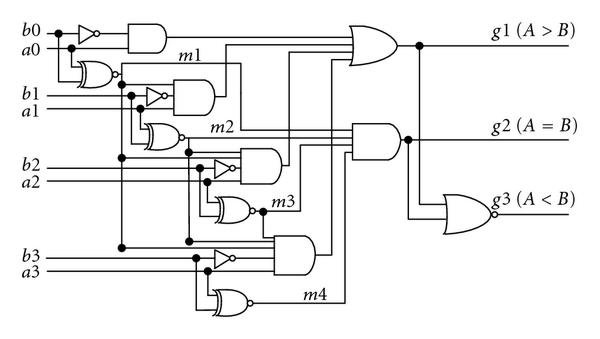
\includegraphics[width=.7\textwidth]{parts/chap-3/img/yao-comp.jpg}
    \caption{The figital comporator is the boolean circuit used to soleve Yao's millionnaire problem.} 
    \label{c2:yao-comp}
\end{figure}

This protocol executes in polynomial time, but there exists a lots of optimisations that allow to garble and evaluate the gates more rapidly.

\subsubsection{GMW protocol}
The \emph{Goldreich-Micali-Widgerson} (GMW) protocol can be seen as an extension of garbled circuits to multiple parties using Yao's idea of using oblivious transfer \cite{Goldreich1987HowGame}. The main principles here are based upon bit-sharing: each party shares its input bits among the $n$ players $b = \sum_{i=1\ldots n}b_i \mod 2$. Each player then processes their shares among the circuit. XOR-gates are easy as they can just addition the shares $c_i = a_i + b_i$. However AND-gates are more tricky: we can see from the decomposition that $c = a \cdot b = \sum_{i\neq j}a_ib_j+\sum_{1\leq i< j\neq n}\left(a_ib_j + a_jb_i \right) \mod 2$. By consequence, each party will have to compute $a_ib_i+ \sum_{i\neq j}\left( a_ib_j + a_jb_i\right)$. As for the XOR-gate, the first part is trivial to evaluate, however, the second cannot be computed by party $i$ without more information from party $j$. This is solved by using a variant of garbled circuits with oblivious transfer between parties $i$ and $j$.

\subsection{Avoiding bit-wise decomposition}
Alternatively, some arithmetic circuits can also be used for multi-party computation. The problem of the bit-wise decomposition and the use of the boolean circuit transcription of the function we jointly want to evaluate is their expensiveness in terms of performance. Indeed, a simple operation can rapidly lead to a lot of gates. For example, let's consider the addition of two number: for two numbers of $n$ bits, the total number of gates is $5n$ in a full adder composition. This is even worse for multiplication. Of course, some optimisations can be made, but the general number of gates is very high compared to the arithmetic circuit of the same function, where it would just be one single gate for addition and multiplication. We will see later that MPC over arithmetic circuits has a much higher \emph{round complexity} --- the dependence of the different rounds on each other --- which leads to less possible parallelisation than with boolean circuits. Nevertheless, one can argue that the parallelisation of bit-wise decomposition does not compensate the much higher number of gates and is thus less efficient than arithmetic circuits in general \cite{Aly2018PracticallyBit-Decomposition}.

+ general comparison of bit-wise decomposition performance and additive secret sharing comparison \cite{Blom2014AThesis}.

Comparisons are much more feasible in boolean circuits.

\subsubsection{How to share a secret}
The building block of multi-party computation over arithmetic is based upon secret sharing. Each party computes its own version of the circuit with the shares of the different parties. At the end of the circuit processing, each party has a share of the final output, which can then be put together to obtain the final output. We first have to define a way for a party to share its secret among $n$ parties, including itself.

\paragraph{Additive secret sharing}
The simplest idea is just to divide the secret $a$ in $n$ shares $a_i$ using a simple summation: $a = \sum_{i=1 \ldots n}a_i$. However, doing it in this manner allows the shares to release some information about the secret, as the shares are not random and strongly depend on the secret. They are two solutions to this problem and the first one is to consider additive sharing over $\mathbb{Z}_q$. The sharing now becomes $a = \sum_{i=1\ldots n}a_i \mod q$ which solves the problem, as the shares can now really be chosen at random. The other solution is over $\mathbb{Z}$ and consists in choosing a sufficiently large interval in which the shares are chosen to dilute sufficiently the statistical information about the secret, typically $a_i \in \left[-A2^\rho,A2^\rho\right]$ with $A$ the size of the interval of the secret $a \in \left[-A,A\right]$ and typically $\rho=128$.

Another consequence of this scheme is that all parties are vital to the recovery of secret as a loss of one secret unables us to reconstruct the secret or any statistical information about it as we took care of that. The scheme does not tolerate the loss or treason of one party and is therefore very sensitive to any failure or malicious player. This problem is solved by polynomial secret sharing.



\paragraph{Polynomial secret sharing}
The idea of polynomial sharing was originally proposed by Shamir in 1979 \cite{Shamir1979HowSecret}. This method allows $n$ parties to share a secret in a way such that any subset of $t+1$ parties can later reconstruct the secret but any subgroup of maximum $t$ parties can do so. The scheme is based on the single fact that for any polynomial of degree $d$, any subset of $d+1$ or more different points can reconstruct the polynomial completely whereas any subset of at most $d$ points is left with an infinite number of possibilities.

The scheme goes as follows. The party that wants to share its secret first constructs a polynomial of degree $t$.
\begin{equation}
    h(z) = a + \sum_{i=1}^t b_i z^i
\end{equation}
with secret $a$ random coefficients $b_i$. For the same reasons as for additive secret sharing, the coefficients can either be chosen in $b_i \in \mathbb{Z}_q$ (which also leads to the consideration of polynomial $h(z) \mod q$ instead), either in the interval $b_i \in \left[-A2^\rho,A2^\rho\right]$.
\noteH{should I demonstrate ?}

We verify that $h(0)=a$ and distribute shares $a_i$ to each party $i$ --- including ourselves --- as follows $a_i=h(i)$. $t+1$ parties can now reconstruct the polynomial together using e.g. Lagrange's polynomials and compute $f(0)$ to recover the secret share. An interesting property is that the recovery can be done as a simple linear combination. Indeed, we have
\begin{eqnarray*}
    h(0) &=& \sum_{i=1}^{n} l_i(0)h(i) \\
    a &=& \sum_{i=1}^{n} r_ia_i
\end{eqnarray*}
where $r = \left(r_1, \ldots , r_n\right) = \left(l_1(0), \ldots , l_n(0)\right)$ is called the \emph{recombination vector} with $l_i(z)$ the $i$-th order Lagrange polynomial, for example
\begin{equation*}
    l_i(z) = \prod_{1\leq j \leq n,j\neq i}\frac{z-j}{i-j}
\end{equation*}
This also works with any generating set of $\mathbb{Z}\left[z\right]$ (or alternatively $\mathbb{Z}_q\left[z\right]$), as long all parties use the same set.

\subsubsection{Performing basic operations}

\paragraph{Addition and multiplication of public constants}
Each party just adds or multiplies his share with the constant. This rests on some arithmetic properties of polynomials: one can easily verify that $a_i+c$ is a share of $a+c$ and $c \cdot a_i$ of $c \cdot a$.

\paragraph{Addition of two secrets}
Let's consider the addition of two polynomials: the respective coefficients just add up. By consequence, two secrets $a$ and $b$ can be added up if every party adds their local shares $a_i+b_i$.
\noteH{False, the values $h(i)$ are added up, not the coefficients}


\paragraph{Multiplication of two secrets}
Unfortunately, it is not possible to adopt the same strategy for multiplication as the multiplication of two polynomials of order $t$ will lead to a new polynomial of order $2t$ which will double the number of parties needed to recover the secret output. In real-case functions with a lot of multiplications, this becomes rapidly impracticable and theoretically unsolvable if the degree of the new polynomial exceeds $n$. Another problem is of statistical order: the new polynomial is not random anymore as it is for example not irreducible anymore by construction. Different algorithms exist to solve this problem \noteH{cite different algorithms ?}

\paragraph{Exponentiation}


\paragraph{Boolean operations}
\section{Protocols implemented}
As said before, we aim here at evaluating a data query of a first party against the database of a second party using various machine-learning algorithms. The goal here is to preserve the privacy of the data of both parties. In the following sections, $\secret{a}_i$ and $\secret{a}_{ij}$ denote a secret in matrix (or array) of secrets and should not be confused with $\secret{a_i}$ which denote a share of the secret in the previous sections. $\secret{A}$ denotes the corresponding matrix. Similarly, we use the notation $\secret{A}_{i:}$ or  $\secret{A}_{:j}$ to denote the vector corresponding to the $i$-th line or $j$-th column of the matrix of secret values.

\subsection{Principal component analysis}
Let us consider the matrix of the PCA weights $W_{n_p , n_f}$ and a list of queries to be transformed $X_{n_q , n_f}$ were $n_p$ the number of principal components, $n_q$ is the number of queries and $n_f$ the number of features. Transforming these queries into the principal components scores $T_{n_q , n_p}$ described in $W$ just corresponds to the matrix multiplication operation $T=X \cdot W^T$. This operation is securely implemented in algorithm~\ref{alg:sec-pca}.

As we can see, this simple matrix multiplication has the theoretical computational complexity of the naive matrix multiplication algorithm $\mathcal{O}(n_q n_p n_f)$ which is cubic.

There is here total secrecy on the values of the queries and the PCA weights. The only public information are the indices of the loops, but at each operation, a totally opaque operation occurs. To summarize, the secrecy is preserved for all the data except its sizes: the number of principal components kept $n_p$, the number of queries $n_q$ and the number of features $n_f$.

\begin{center}
\begin{algorithm}[H]
\KwData{$n_p \times n_f$ matrix of principal components weights $\secretF{W}$ and $n_q \times n_f$ matrix of queries $\secretF{X}$.}
\KwResult{$n_q \times n_p$ matrix of the $n_p$ first components scores of each query $\secretF{T}$.}
\DontPrintSemicolon
initialize $\secretF{T}$ of size $n_q \times n_p$ \;
\ForEach{$i = 1, \ldots, n_q$}{
\ForEach{$j = 1,\ldots, n_p$}{
\ForEach{$k = 1, \ldots, n_f$}{
$\secretF{t}_{ij} \leftarrow \secretF{t}_{ij} + \secretF{w}_{jk} \cdot \secretF{x}_{ik}$ \;
}
}
}
\Return{$\secretF{T}$}
\caption{The secret PCA evaluation protocol.}
\label{alg:sec-pca}
\end{algorithm}
\end{center}

%%%%%%%%%%%%%%%%%%%%%%%%%%%%%%%%%%%%%%%%%%%%%%%%%%%%%%%%%%%%%%%%%%%%%%%%%%%%%%%%%%%%%%%%%%%%%%%%%%%%%%%%%%%%%%%
\subsection{Linear support vector machines}
The linear support vector machine protocol is basically the same as the PCA evaluation protocol as it also consists in a matrix multiplication, with the difference that an intercept vector has to be added. The protocol evaluates a linear support vector machine in its primal form which consists of a scalar product that sees a constant added to it. However, as we work with multi-class support vector machines, we have to consider multiple scalar products and similarly, as we work with more than one query, this corresponds to a matrix multiplication in total.

Let us consider now a matrix $W_{n_c,n_f}$ where $n_c$ is the number of classes --- each SVM represents one class --- that contains the primal weights of the linear support vector machine. To that we have to add the intercept vector $B_{n_c}$. The list of queries is the same as before $X_{n_q , n_f}$. The output is a matrix containing the score of for each query on each SVM $S_{n_c,n_q}$. The operation becomes $S = WX^T + B$. The protocol implementing it is given at algorithm~\ref{alg:sec-lsvm}.

The complexity here is similar as before $\mathcal{O}(n_c n_q n_f)$. If we use feature space reduction and the queries are first transformed using the principal component analysis ($n_f$ is reduced to $n_p$), it becomes $\mathcal{O}(n_c n_q n_p)$. However, we eventually have to add the complexity of the PCA evaluation which gives a total of $\mathcal{O}(n_p n_q (n_f+n_c)) > \mathcal{O}(n_c n_q n_f)$ for $n_f,n_c \geq 1$ which is always verified. Hence, we should not expect the linear support vector machines to be more effective using a PCA feature reduction. However, this is not the case for the $\chi^2$-feature reduction linear support vector machine where the complexity is always slower than the full-feature linear support vector machine. Indeed, we have $\mathcal{O}(n_c n_q n_{\chi^2}) < \mathcal{O}(n_c n_q n_f)$ if $n_{\chi^2} < n_f$ which should be the case for a working $\chi^2$ feature selection.

Here again, the secrecy is preserved in all the data except the sizes, adding here the size $n_c$ of the $\chi^2$ features kept to the ones already discussed in the subsection above. We could decide to hide $n_c$ by just using a null SVM weight for a coefficient that has been dropped by the selection, but this would not allow to reduce the complexity. This is of no interest as the whole idea of $\chi^2$ feature selection is to increase the evaluation speed.

\begin{center}
\begin{algorithm}[H]
\KwData{$n_c \times n_f$ matrix of the $n_c$ different SVM weights $\secretF{W}$, $n_q \times n_f$ matrix of queries $\secretF{X}$ and an intercept vector $\secretF{B}$ of length $n_c$.}
\KwResult{$n_c \times n_q$ matrix containing the $n_c$ SVM scores for each query $\secretF{S}$.}
\DontPrintSemicolon
initialize $\secretF{T}$ of size $n_q \times n_p$ \;
\ForEach{$i = 1, \ldots, n_q$}{
\ForEach{$j = 1,\ldots, n_c$}{
\ForEach{$k = 1, \ldots, n_f$}{
$\secretF{s}_{ji} \leftarrow \secretF{s}_{ji} + \secretF{w}_{jk} \cdot \secretF{x}_{ik}$ \;
}
$\secretF{s}_{ji} \leftarrow \secretF{s}_{ji} + \secretF{b}_j$ \;
}
}
\Return{$\secretF{S}$}
\caption{The secret linear SVM evaluation protocol.}
\label{alg:sec-lsvm}
\end{algorithm}
\end{center}

%%%%%%%%%%%%%%%%%%%%%%%%%%%%%%%%%%%%%%%%%%%%%%%%%%%%%%%%%%%%%%%%%%%%%%%%%%%%%%%%%%%%%%%%%%%%%%%%%%%%%%%%%%%%%%%
\subsection{Support vector machines with radial based functions}
As a reminder the evaluation of a query $x$ on linear support vector using a kernel functions only is possible in the dual space and is given by
\begin{equation}
    \mathtt{SVM}(x) = \sum_{i=1}^{n_s} \alpha_i y_i K(x_i,x) + b
\end{equation}
where $x_i$ are the $n_s$ support vectors $x_i$ and $K(x_i,x)$ the kernel function here given by
\begin{equation}
    K\left( x_i,x_j\right) = \exp\left(-\frac{\norm{x_i - x_j}^2}{2\sigma^2}\right)
\end{equation}
With $\sigma^2$ a kernel parameter. Unfortunately, SCALE-MAMBA has no support for exponentiation of secret fixed point integers. This can be easily circumvented using a Taylor expansion of the exponential function
\begin{equation}
    e^x \approx \sum_{n=0}^{n_e} \frac{x^n}{n!}
\end{equation}
with $n_e$ the number of iterations we want to perform (the more the better), but does not allow us to use more effective methods based on square pairs for example for classical exponentiation. The secure radial based kernel function protocol is developed in algorithm~\ref{alg:sec-kernel} using the secure distance computation protocol described in algorithm~\ref{alg:sec-dist}. Once these protocols are defined, we can use the protocol described at algorithm~\ref{alg:sec-rbfsvm} to compute the transformation of the queries into the dual space, which is equivalent to the kernel matrix between the support vectors and the queries. These transformed queries can then be used with the classical linear support vector machines, but with the dual $\alpha_i$ coefficients instead of the primal weights which changes the $n_f$ estimations to $n_s$ in the protocol described at algorithm~\ref{alg:sec-lsvm}. Though, one dual transformation is needed per different SVM.

Let's now have a look at the complexity. The complexity of the transformation is $\mathcal{O}(n_fn_en_s)$ per SVM. As they are $n_c$ different SVMs, this gives $\mathcal{O}(n_cn_fn_en_s)$ for all the transformations. If we add the estimation of the SVMs themselves based on these dual transformations, this gives a total of $\mathcal{O}(n_cn_s(n_q+n_en_f))$. The use of support vectors in the dual makes the complexity of degree 4 and not cubic anymore. The next chapter aims at investigating if this trade-off is worth the cost.

Similarly as before, we can also use a PCA transformation before the computation of the support vectors and try to gain speed on the distance computation. As we saw before, the PCA transformation has a cubic complexity and this should thus not change the degree of the estimation, but reduce its factors to $\mathcal{O}(n_cn_s(n_q+n_en_p))$ where $n_p$ is the number of components kept. Computationally speaking, this trade-off here is expected to deliver better results. Using $\chi^2$ selection reduces the complexity to $\mathcal{O}(n_cn_s(n_q+n_en_{\chi^2}))$ which should also deliver better results. The choice between PCA and $\chi^2$ feature selection was trivially favouring the latter for the linear SVM in every case, here it tends to favor the first one if $n_p<n_{\chi^2}$ as the computation PCA evaluation has no significant influence on the complexity here, which was not the case here above.

\begin{center}
\begin{algorithm}[H]
\KwData{secret vector $\secretF{U}$ of size $n_f$ and secret vector $\secretF{V}$ of same size.}
\KwResult{$\secretF{d}$ corresponding to $d = \norm{U-V}^2$.}
\DontPrintSemicolon
\ForEach{$i = 1,\ldots,n_f$}{
$\secretF{d} \leftarrow \secretF{d} + (\secretF{u}_i-\secretF{v}_i)^2$ \;
}
\Return{$\secretF{d}$}
\caption{The secret distance computation protocol $\mathtt{Dist}$.}
\label{alg:sec-dist}
\end{algorithm}
\end{center}

\begin{center}
\begin{algorithm}[H]
\KwData{secret vector $\secretF{U}$ of size $n_f$, secret vector $\secretF{V}$ of same size and secret kernel parameter $\secretF{a}$ sharing $2\sigma^2$.}
\KwResult{$\secretF{d}$ corresponding to $K(u,v)$ with parameter $2\sigma^2$.}
\DontPrintSemicolon
$\secretF{v} \leftarrow - \mathtt{Dist}(\secretF{U},\secretF{V}) / \secretF{a}$ \;
\ForEach{$i=0,\ldots,n_e$}{
$\secretF{d} \leftarrow \secretF{d} + \secretF{v}^i/i!$
}
\Return{$\secretF{d}$}
\caption{The secret radial based kernel function evaluation protocol $\mathtt{Kernel}$.}
\label{alg:sec-kernel}
\end{algorithm}
\end{center}

\begin{center}
\begin{algorithm}[H]
\KwData{secret matrix of queries $\secretF{X}$ of size $n_q \times n_f$, secret matrix of support vectors $\secretF{S}$ of size $n_s \times n_f$ and secret kernel parameter $\secretF{a}$.}
\KwResult{$\secretF{T}$ transformed queries into the dual space.}
\DontPrintSemicolon
initialize $\secretF{T}$ of size $n_q \times n_s$ \;
\ForEach{$i = 1,\ldots, n_q$}{
\ForEach{$j = 1,\ldots, n_s$}{
$\secretF{t}_{ij} \leftarrow \mathtt{Kernel}(\secretF{X}_{i:},\secretF{S}_{j:},\secretF{a})$ \;
}
}
\Return{$\secretF{T}$}
\caption{The secret dual space transformation protocol.}
\label{alg:sec-rbfsvm}
\end{algorithm}
\end{center}

%%%%%%%%%%%%%%%%%%%%%%%%%%%%%%%%%%%%%%%%%%%%%%%%%%%%%%%%%%%%%%%%%%%%%%%%%%%%%%%%%%%%%%%%%%%%%%%%%%
\subsection{Multi-class evaluation}
The SVMs only perform binary classification and are combined to perform multi-class classification. To evaluate the one-against-all model, we just have to take the maximum score of each SVM and return the corresponding target. In the protocol described in algorithm~\ref{alg:sec-multi1}, the final score of the wining SVM is not returned and sole the corresponding class is. In the following algorithms, the notation $\secretF{-\infty}$ describes a very small value that is certainly smaller than all SVMs scores (these are typically comprised between -1 and 1 and a value of -1000 suffices). In the very unlikely case where no score is bigger than this value, the algorithm will return the secret index 0. The complexity of the algorithm is equal to $\mathcal{O}(n_qn_c)$ but incorporates for the first time comparisons.

Similarly, we can define the algorithm picking the winner for a tree-based model. This is done by picking the index of the highest SVM in the tree returning a positive score. Once a SVM returns a positive score, all next scores become not relevant. However, to preserve the security, we still need to evaluate all SVMs and cannot stop even if the SVM higher in the tree returned one. If we did this, an attacker could just look at the index of the SVM when the algorithm stops to disclose the winning target. The protocol for defining the winning target in the case of a tree-based multi-class model is given at algorithm~\ref{alg:sec-multi2}. In this case, it is not possible that the algorithm returns 0 and finds no winner. The computational complexity is exactly the same as the one-against-all, but $n_c = 4$ and not to 5.

\begin{center}
\begin{algorithm}[H]
\KwData{$n_c \times n_q$ matrix containing the $n_c$ SVM scores for each query $\secretF{S}$ and an integer vector corresponding to index of the classes $\secretI{C}$ of size $n_c$.}
\KwResult{vector $\secretI{N}$ of size $n_q$ containing the winning indices for each query.}
\DontPrintSemicolon
initialize vector $\secretI{N}$ of size $n_q$ to $\secretI{0}$ \;
\ForEach{$i=1,\ldots,n_q$}{
$\secretF{m} \leftarrow \secretF{\infty}$ \;
\ForEach{$j = 1,\ldots,n_c$}{
$\secretI{b} \leftarrow \secretF{S}_{ji} > m$ \;
$\secretF{m} \leftarrow_{\secretI{b}} \secretF{S}_{ji} : m$ \;
$\secretI{N}_i \leftarrow_{\secretI{b}} \secretI{C}_j : n$ \;
}
}
\Return{$\secretI{N}$}
\caption{The secret one-against-all multi-class evaluation protocol.}
\label{alg:sec-multi1}
\end{algorithm}
\end{center}

\begin{center}
\begin{algorithm}[H]
\KwData{$n_c \times n_q$ matrix containing the $n_c$ SVM scores for each query $\secretF{S}$ and an integer vector corresponding to index of the classes $\secretI{C}$ of size $n_c$.}
\KwResult{vector $\secretI{N}$ of size $n_q$ containing the winning indices for each query.}
\DontPrintSemicolon
initialize vector $\secretI{N}$ of size $n_q$ \;
\ForEach{$i=1,\ldots,n_q$}{
\ForEach{$j = n_c,\ldots,1$}{
$\secretI{b} \leftarrow \secretF{S}_{ji} > 0$ \;
$\secretI{N}_i \leftarrow_{\secretI{b}} \secretI{C}_j : n$ \;
}
}
\Return{$\secretI{N}$}
\caption{The secret tree-based multi-class evaluation protocol.}
\label{alg:sec-multi2}
\end{algorithm}
\end{center}


%%%%%%%%%%%%%%%%%%%%%%%%%%%%%%%%%%%%%%%%%%%%%%%%%%%%%%%%%%%%%%%%%%%%%%%%%%%%%%%%%%%%%%%%%%%%%%%%%
\subsection{Nearest neighbours}
The secure evaluation of the $k$-NN protocol happens in two phases, the first one is computing the distances between the query and the different points of the training size $n_t$. This is done using the protocol described in algorithm~\ref{alg:sec-dist}. The points are then ordered and the winning target is returned. Here again, the smallest distance is not returned to avoid attacks where someone would send a lot of queries of data-points near a certain secret point of the training data-set and try to triangulate its position\footnote{As we are working in a feature space of dimension $d$, $d+1$ points are still needed for triangulation in the favorable case where all these points are the closest to the targeted point and return their distance to it and not another closer point.}.

There are different possibilities for implementing the algorithm (we use a minimum selection algorithm with complexity $\mathcal{O}(n\log n)$:
\begin{itemize}
    \item The first idea is to compute all distances which has a complexity $\mathcal{O}\left(n_tn_f\right)$ and then go $k$ times through those distances to find the $k$ smallest ones, which has complexity $\mathcal{O}\left(ln_t\log n_t\right)$. This algorithm, which calculates the distances, stores them and go $k$ times through them has total complexity $\mathcal{O}\left(n_tn_f+kn_t\log n_t \right)$, but requires $\mathcal{O}\left(n_t\right)$ extra memory.
    \item An alternative could be to avoid the storing of the distances and compute them during the classifying. The algorithm goes $k$ through all observations as before, but computes the distance at that moment. The advantage is the requirement of no extra memory, however the computational complexity becomes $\mathcal{O}\left(n_fkn_t \log n_t\right)$.
    \item A third alternative could be to use Hoare's \emph{quickselect} algorithm \cite{Hoare:1961:AF:366622.366647}. This algorithm is able to find the $k$\textsuperscript{th} smallest --- alternatively biggest --- elements of a list in best case scenario $\mathcal{O}\left(n_t\right)$ and worst case scenario $\mathcal{O}\left(n_t \log n_t\right)$. The practice shows that the algorithm tends to obtain a complexity closer to the best case than the worst case scenario. Using this algorithm, one could hope to obtain a $k$-NN computational complexity of $\mathcal{O}\left(n_tn_f\right)$. Unfortunately, this algorithm uses recursive function calls which are currently not supported in the SCALE-MAMBA framework. More discussion is given in the next sections and in appendix~\ref{app:qs}. As the indices are not secret, this would also reveal part of the sorting pattern, but as the distances are not revealed, triangulation-based attacks would still not be possible.
\end{itemize}
As storing is not really a concern in secret sharing, but the bottleneck is the computation part. The first option has been chosen. The secure $k$-NN evaluation protocol is given at algorithm~\ref{alg:sec-knn} for a unique query. One just has to rerun it $n_q$ times to compute multiple queries. This protocol rests on two other sub-protocols, the first one aims at defining the majority class present in the neighbours and is described at algorithm~\ref{alg:sec-win}. It first consists in a counting of the elements present in the neighbours and searching for the maximum. In case of tie, the highest value tied class is returned. This choice is made to limit the number of false negatives\footnote{This depends on the data-set used in the next chapter. In that data-set the higher classes tend to be more difficultly recognizable. This case is also to be nuanced as the algorithm as we will see performs the best for $k=1$ where no ties are possible.}.

When $k=1$, the part of the algorithm where the majority voting is used can be dropped as well as the need for selecting a minimum higher to the one previously found (which comprises two time more comparisons). For this purpose, two protocols for the computation of a minimum are given. One for the $k=1$ case at algorithm~\ref{alg:sec-min1} and another for $k>1$ at algorithm~\ref{alg:sec-min2}. The reason we have to use a specific protocol for the selection of an minimum when a threshold (the previous minimum for $k-1$) is because it is not possible to modify the current distance array to change the value of the previously found distance or just to suppress that element without revealing its index. Both protocols have complexity $\mathcal{O}(n_t \log n_t)$. For the sake of simplicity, they are referred to by the same name.

The complexity of the protocol for $n_q$ queries is $\mathcal{O}(n_q\{n_tn_f + kn_t \log n_t\})$, $\mathcal{O}(n_q\{n_p(n_t+n_f) + kn_t \log n_t\})$ with PCA feature reduction and $\mathcal{O}(n_q\{n_tn_{\chi^2} + kn_t \log n_t\})$ with $\chi^2$ feature selection.

\begin{center}
\begin{algorithm}[H]
\KwData{query vector $\secretF{X}$ of size $n_f$, matrix of training points $\secretF{P}$ of size $n_t \times n_f$ and corresponding classes vector of $\secretI{C}$ of size $n_t$.}
\KwResult{class $\secretI{l}$ for the query.}
\DontPrintSemicolon
initialize vector $\secretF{D}$ of size $n_q$ \;
\ForEach{$i=1,\ldots,n_t$}{
$\secretF{d}_i \leftarrow \mathtt{Dist}(\secretF{X},\secretF{P}_{i:})$ \;
}
$\secretF{m} \leftarrow \secretI{-\infty}$ \;
initialize vector $\secretI{T}$ of size $k$ \;
\ForEach{$i=1,\ldots,k$}{
$\secretI{t}_i, \secretF{m} \leftarrow \mathtt{Min}(\secretF{D},\secretI{C},\secretF{m})$ \;
}
$\secretI{l} \leftarrow \mathtt{MajVote}(\secretI{T})$ \;
\Return{$\secretI{l}$}
\caption{The secret $k$-NN evaluation protocol.}
\label{alg:sec-knn}
\end{algorithm}
\end{center}

\begin{center}
\begin{algorithm}[H]
\KwData{vector $\secretI{T}$ containing the targets of the $k$ nearest neighbours.}
\KwData{$\secretI{l}$ containing the most present target. In case of a tie, the highest tied class is returned.}
\DontPrintSemicolon
initialize vector $\secretI{r}$ of size $n_c$ to 0\;
\ForEach{$i=1,\ldots,n_c$}{
\ForEach{$j=1,\ldots,k$}{
$\secretI{b} \leftarrow \secretI{t}_j = i$ \;
$\secret{r}_i \leftarrow_{\secretI{b}} \secret{r}_i + 1 : \secret{r}_i$ \;
}
}
$\secretI{l} \leftarrow 0$ \;
$\secretI{c} \leftarrow 0$ \;
\ForEach{$i=1,\ldots,n_c$}{
    $\secretI{b} \leftarrow \secret{r}_i \geq \secretI{y}$ \;
    $\secretI{c} \leftarrow_{\secretI{b}} \secret{r}_i : c$ \;
    $\secretI{l} \leftarrow_{\secretI{b}} i : l$ \;
}
\Return{$\secretI{l}$}
\caption{The majority vote evaluation protocol $\mathtt{MajVote}$.}
\label{alg:sec-win}
\end{algorithm}
\end{center}


\begin{center}
\begin{algorithm}[H]
\KwData{vector of distances $\secretF{D}$ of size $n_t$ and corresponding classes $\secretI{C}$.}
\KwResult{shortest distance $\secretF{d}$ and corresponding class $\secretI{c}$.}
\DontPrintSemicolon
\If{$n_t=1$}{
\Return{$\secretF{d}_1, \secret{c}_1$}
}
\Else{
$n' \leftarrow \lfloor (n_t+1)/2 \rfloor$ \;
initialize $\secretF{D'}$ of size $n'$ \;
initialize $\secretI{C'}$ of size $n'$ \;

\ForEach{$i=1,\ldots,\lfloor n_t/2\rfloor$}{
$\secretI{b} \leftarrow \secretF{d}_{2i} < \secretF{d}_{2i+1}$ \;
$\secretF{d'}_i \leftarrow_{\secretI{b}} \secretF{d}_{2i} : \secretF{d}_{2i+1}$ \;
$\secretF{c'}_i \leftarrow_{\secretI{b}} \secretF{c}_{2i} : \secretF{c}_{2i+1}$ \;
}
\If{n \mod 2 = 1}{
$\secretF{d'}_{n'-1} \leftarrow \secretF{d}_{n_t-1}$ \;
$\secretF{c'}_{n'-1} \leftarrow \secretF{c}_{n_t-1}$ \;
}
\Return{$\mathtt{Min}(\secretF{D'},\secretF{C'})$}
}
\caption{The secret minimum evaluation protocol $\mathtt{Min}$ ($k=1$).}
\label{alg:sec-min1}
\end{algorithm}
\end{center}


\begin{center}
\begin{algorithm}[H]
\KwData{vector of distances $\secretF{D}$ of size $n_t$, corresponding classes $\secretI{C}$ and minimum threshold $\secretF{m}$.}
\KwResult{shortest distance $\secretF{d}$ and corresponding class $\secretI{c}$.}
\DontPrintSemicolon
\If{$n_t=1$}{
\Return{$\secretF{d}_1, \secret{c}_1$}
}
\Else{
$n' \leftarrow \lfloor (n_t+1)/2 \rfloor$ \;
initialize $\secretF{D'}$ of size $n'$ \;
initialize $\secretI{C'}$ of size $n'$ \;

\ForEach{$i=1,\ldots,\lfloor n_t/2\rfloor$}{
$\secretI{b} \leftarrow \secretF{d}_{2i} < \secretF{d}_{2i+1}$ \;
$\secretF{d''} \leftarrow_{\secretI{b}} \secretF{d}_{2i} : \secretF{d}_{2i+1}$ \;
$\secretF{c''} \leftarrow_{\secretI{b}} \secretF{c}_{2i} : \secretF{c}_{2i+1}$ \;
$\secretF{d'''} \leftarrow_{\secretI{b}} \secretF{d}_{2i+1} : \secretF{d}_{2i}$ \;
$\secretF{c'''} \leftarrow_{\secretI{b}} \secretF{c}_{2i+1} : \secretF{c}_{2i}$ \;
$\secretI{b'} \leftarrow \secretF{d''} > \secretF{m}$ \;
$\secretF{d'}_i \leftarrow_{\secretI{b'}} \secretF{d''} : \secretF{d'''}$ \;
$\secretF{c'}_i \leftarrow_{\secretI{b'}} \secretF{c''} : \secretF{c'''}$ \;
}
\If{n \mod 2 = 1}{
$\secretF{d'}_{n'-1} \leftarrow \secretF{d}_{n_t-1}$ \;
$\secretF{c'}_{n'-1} \leftarrow \secretF{c}_{n_t-1}$ \;
}
\Return{$\mathtt{Min}(\secretF{D'},\secretF{C'})$}
}
\caption{The secret minimum evaluation protocol with threshold $\mathtt{Min}$ ($k>1$).}
\label{alg:sec-min2}
\end{algorithm}
\end{center}

\chapter{Experimental results and discussion}

\section{The NSL-KDD dataset}
\section{Support Vector Machines}
\section{Nearest neighbours}

\subsection{Algorithms and complexity}
The distances are then sorted to find the $k$ smallest ones. This can be done in different manners:
\begin{itemize}
    \item The first idea is to compute all distances which has a complexity $\mathcal{O}\left(nd\right)$ and then go $k$ times through those distances to find the $k$ smallest ones, which has complexity $\mathcal{O}\left(nk\right)$. This algorithm, which calculates the distances, stores them and go $k$ times through them has total complexity $\mathcal{O}\left(nd+nk\right)$, but requires $\mathcal{O}\left(n\right)$ extra memory
    \item An alternative could be to avoid the storing of the distances and compute them during the classifying. The algorithm goes $k$ through all observations as before, but computes the distance at that moment. The advantage is the requirement of no extra memory, however the computational complexity becomes $\mathcal{O}\left(ndk\right)$.
    \item A third alternative could be to use Hoare's \emph{quickselect} algorithm \cite{Hoare:1961:AF:366622.366647}. This algorithm is able to find the $k$\textsuperscript{th} smallest --- alternatively biggest --- elements of a list in best case scenario $\mathcal{O}\left(n\right)$ and worst case scenario $\mathcal{O}\left(n \log n\right)$. The practice shows that the algorithm tends to obtain a complexity closer to the best case than the worst case scenario. Using this algorithm, one could hope to obtain a $k$-NN computational complexity of $\mathcal{O}\left(nd\right)$. In more details, the algorithm uses an auxiliary subroutine that reorganises a given partition --- specified by two indices --- into elements smaller than a given pivot point left of it and bigger, right of it. The main algorithm then makes recursive calls to that same subroutine until the pivot ends at the $k$\textsuperscript{th} position. The algorithm and its subroutine are given at \ref{alg:knn-1} and \ref{alg:knn-2}.
\end{itemize}

\begin{center}
\begin{algorithm}[H]
 \KwData{list $\left\{y_i\right\}$, partition start index $i_{a}$, partition end index $i_{b}$, pivot index $i_{p}$}
 \KwResult{new pivot index $j_p$, sorted list $\left\{y_j\right\}$ of $\left\{y_{i_{a}} , \ldots , y_{i_{b}}\right\}$ where $\forall j < j_{p} : y_j < y_{i_{p}}$, $\forall j > j_{p} : y_j > y_{i_{p}}$ and $y_{j_{p}} = y_{i_{p}}$}
 \DontPrintSemicolon
  \SetKwFunction{FPartition}{partition}
  \SetKwProg{Fn}{function}{:}{}
  \Fn{\FPartition{$\left\{y_i\right\}$, $i_a$, $i_b$, $i_p$}}{
 $p \leftarrow y_{i_{p}}$\;
 $l \leftarrow a$\;
 \For{ $i = i_a$ \KwTo $i_b-1$}{
  \If{$y_i < p$}{
   swap $y_i$ and $y_k$\;
   $k \leftarrow k+1$\;
   }
   swap $y_b$ and $y_k$
 }
 $j_p \leftarrow l$\;
 \Return{$j_p$, $\left\{y_j\right\}$}}
 \caption{Quickselect's partition subroutine}
 \label{alg:knn-1}
\end{algorithm}
\end{center}

\begin{center}
\begin{algorithm}[H]
 \KwData{list $\left\{y_i\right\}$, partition start index $i_{a}$, partition end index $i_{b}$, number of smallest elements wanted $k$}
 \KwResult{new list $\left\{y_j\right\}$ containing $k$ smallest elements}
 \DontPrintSemicolon
  \SetKwFunction{FSelect}{select}
  \SetKwFunction{FPartition}{partition}
  \SetKwProg{Fn}{function}{:}{}
  \Fn{\FSelect{$\left\{y_i\right\}$, $i_a$, $i_b$, $k$}}{
\eIf{$i_a = i_b$}{
\Return $\left\{y_1 , \ldots , y_{i_a}\right\}$}{
$l, \left\{y_j\right\} \leftarrow$ \FPartition{$\left\{y_i\right\}$, $i_a$, $i_b$, $l$}
\tcp*[r]{assign random $l$ if not already assigned} \;
\uIf{$k=l$}{
\Return{$\left\{y_1 , \ldots , y_k\right\}$}}
\uElseIf{$k<l$}{
\Return{\FSelect{$\left\{y_i\right\}$, $i_a$, $l+1$, $k$}}}
\uElse{\Return{\FSelect{$\left\{y_i\right\}$, $l+1$, $i_b$, $k$}}}
}
}
 \caption{Quickselect's main routine}
 \label{alg:knn-2}
\end{algorithm}
\end{center}


\subsection{Feature reduction applied to $k$-NN}






\subsection{Combining condensed nearest neighbours with feature reduction}
\section{Ensemble methods}

\chapter{Conclusion}

\appendixpage*
\appendix
\chapter{Matlab}
\label{app:matlab}

\chapter{SCALE}
\label{app:scale}

\chapter{The Quickselect algorithm}
\label{app:qs}
Hoare's \emph{quickselect} algorithm~\cite{Hoare:1961:AF:366622.366647} is able to find the $k$\textsuperscript{th} smallest --- alternatively biggest --- elements of a list in best case scenario $\mathcal{O}\left(n_t\right)$ and worst case scenario $\mathcal{O}\left(n_t \log n_t\right)$ where $n_t$ is the size of the training set. The practice shows that the algorithm tends to obtain a complexity closer to the best case than the worst case scenario. Using this algorithm, one could hope to obtain a $k$-NN computational complexity of $\mathcal{O}\left(n_tn_f\right)$ where $n_f$ is the feature set size. 

It uses an auxiliary subroutine that reorganizes a given partition --- specified by two indices --- into elements smaller than a given pivot point left of it and bigger, right of it. The main algorithm then makes recursive calls to that same subroutine until the pivot ends at the $k$\textsuperscript{th} position. The algorithm and its subroutine are given at \ref{alg:knn-qs-1} and \ref{alg:knn-qs-2} in clear.

For the algorithm to run using MPC, the comparisons of the main routine have to be revealed in order to decide whether or not make a recursive call. The indices $i_a$ and $i_b$ should also be revealed in order to perform the loop of the subroutine. We can however avoid revealing the results of the comparisons of the subroutine by using a secure conditional swap~\cite{Aly2014SecurelyProblems}.

This algorithm has been implemented but the compilation results in an infinite loop. As the MAMBA language first develops all the python code, it develops the function containing the recursive call the that same function and adds it to the SCALE code. It does so with the new call and adds the new recursive call to the SCALE code. This goes on forever. Classical loops are also fully developed. The only way to really execute a loop is to use certain specific calls to specially developed routines that allow real loops on the SCALE code. Unfortunately, no such routines exist for recursive calls.

 The revelation of the comparisons needed to make the (eventual) recursive calls, $i_a$ and $i_b$ would not guarantee the privacy of the algorithm as much information about the relative order of the distances would be revealed. An solution could be to scramble the training set before each evaluation~\cite{QiEfficient}, but at what costs?
 
 Furthermore, the interest for this algorithm has to be nuanced in the case of intrusion detection systems as $k=1$ provides the best results and can already be theoretically achieved in $\mathcal{O}\left(n_t\right)$.

\begin{center}
\begin{algorithm}[H]
 \KwData{list $\left\{y_i\right\}$, partition start index $i_{a}$, partition end index $i_{b}$, pivot index $i_{p}$}
 \KwResult{new pivot index $j_p$, sorted list $\left\{y_j\right\}$ of $\left\{y_{i_{a}} , \ldots , y_{i_{b}}\right\}$ where $\forall j < j_{p} : y_j < y_{i_{p}}$, $\forall j > j_{p} : y_j > y_{i_{p}}$ and $y_{j_{p}} = y_{i_{p}}$}
 \DontPrintSemicolon
  \SetKwFunction{FPartition}{partition}
  \SetKwProg{Fn}{function}{:}{}
  \Fn{\FPartition{$\left\{y_i\right\}$, $i_a$, $i_b$, $i_p$}}{
 $p \leftarrow y_{i_{p}}$\;
 $l \leftarrow a$\;
 \For{ $i = i_a$ \KwTo $i_b-1$}{
  \If{$y_i < p$}{
   swap $y_i$ and $y_k$\;
   $k \leftarrow k+1$\;
   }
   swap $y_b$ and $y_k$
 }
 $j_p \leftarrow l$\;
 \Return{$j_p$, $\left\{y_j\right\}$}}
 \caption{Quickselect's partition subroutine}
 \label{alg:knn-qs-2}
\end{algorithm}
\end{center}

\begin{center}
\begin{algorithm}[H]
 \KwData{list $\left\{y_i\right\}$, partition start index $i_{a}$, partition end index $i_{b}$, number of smallest elements wanted $k$}
 \KwResult{new list $\left\{y_j\right\}$ containing $k$ smallest elements}
 \DontPrintSemicolon
  \SetKwFunction{FSelect}{select}
  \SetKwFunction{FPartition}{partition}
  \SetKwProg{Fn}{function}{:}{}
  \Fn{\FSelect{$\left\{y_i\right\}$, $i_a$, $i_b$, $k$}}{
\eIf{$i_a = i_b$}{
\Return $\left\{y_1 , \ldots , y_{i_a}\right\}$}{
assign random $l \in \left[i_a,i_b\right]$ \;
$l, \left\{y_j\right\} \leftarrow$ \FPartition{$\left\{y_i\right\}$, $i_a$, $i_b$, $l$} \;
\uIf{$k=l$}{
\Return{$\left\{y_1 , \ldots , y_k\right\}$}}
\uElseIf{$k<l$}{
\Return{\FSelect{$\left\{y_i\right\}$, $i_a$, $l+1$, $k$}}}
\uElse{\Return{\FSelect{$\left\{y_i\right\}$, $l+1$, $i_b$, $k$}}}
}
}
 \caption{Quickselect's main routine}
 \label{alg:knn-qs-1}
\end{algorithm}
\end{center}


\chapter{Additional experimental results}
\label{app:add}

\backmatter
%\bibliographystyle{ieeetr}
%\bibliography{misc/references.bib}
\printbibliography

\end{document}
